\documentclass[conference,10pt]{IEEEtran}
\IEEEoverridecommandlockouts
\usepackage{graphicx,booktabs,amsmath,amssymb,multirow,xcolor,url,xspace}
\usepackage[hidelinks]{hyperref}
\hypersetup{pdftitle={로봇 양팔을 위한 에고센트릭 인간 시연}, pdfauthor={Jeong Hwan Lee}}
\usepackage{tikz}
\usetikzlibrary{positioning,arrows.meta}
\usepackage{fontspec}\setmainfont{Times New Roman}\usepackage{xeCJK}\setCJKmainfont[AutoFakeBold=2.5]{AppleMyungjo}\setCJKsansfont[AutoFakeBold=2.5]{Apple SD Gothic Neo}\setCJKmonofont{Apple SD Gothic Neo}\xeCJKsetup{CJKecglue={},CJKspace=true}
\newcommand{\mm}{\,mm\xspace}
\def\UrlBreaks{\do\/\do\_\do\.\do\-}\def\UrlFont{\small\ttfamily}\newcommand{\code}[1]{\path{#1}}
\renewcommand{\appendixname}{부록}

\begin{document}
\title{로봇 양팔을 위한 에고센트릭 인간 시연:\\손 착용 그리퍼에서 로봇 정책까지}
\author{\IEEEauthorblockN{Jeong Hwan Lee}
\IEEEauthorblockA{기술 보고서, 버전 5, 2026년 10월 12일 \quad alnrg2arg@gmail.com\\ 코드, 결과, 샘플 데이터는 요청 시 제공합니다.}}
\maketitle

\begin{abstract}
본 연구는 BrikHMP18이 설계·공개한 오픈소스 손 착용형 UMI 방식 그리퍼 HandUMI(우리가 설계한 장치가 아님)로 기록한 에고센트릭(egocentric)
인간 시연을 reBot B601 양팔 로봇의 정책 학습 데이터로 어디까지 바꿀 수 있는지 살펴본다. 하나의 보고서가 사슬 전체를 다룬다. 수집
장치, 캘리브레이션, 세 가지 메트릭 스케일 원천을 갖춘 단안 손목 자세, 로봇 학습 데이터로의 두 세대 변환, 0.9B 파라미터 X-VLA 모델,
오프라인 평가와 진단 평가, 그리고 배포이다. \emph{쌓기.} 여섯 가지 균형 잡힌 순서로 큐브 세 개를 쌓는 양팔 시연 349개를 수집하였다.
로봇 관절로 리타게팅하면 양팔 세그먼트 561개가 나온다. 이 데이터로 파인튜닝한 모델은 동작 샘플에서 held-out 인간 동작의 방향을
예측하지만(1.2\,s에서 코사인 0.90, 관절 오차는 무동작 예측기보다 13--32\% 낮음) 정지 구간에서는 드리프트하며, 순서 지시문을 바꾸어도
예측이 더 정확해지지 않는다. 대신 에피소드 전체를 로봇 자신의 상대 데카르트(Cartesian) 액션 계약으로 변환하면 실현 가능성 필터 없이
에피소드 330개가 남는다. 이 계약 아래에서 남은 격차는 시각적이다. 에고 전용 모델은 로봇 프레임에서 유용한 동작 방향을 주지 못하며
(코사인 중앙값 $-0.05$/$-0.03$, 로봇으로 학습한 모델은 $+0.81$/$+0.77$), 격차는 손목 이미지를 따른다. 로봇 파인튜닝의 초기값으로 쓰면
에고 사전학습은 초기 학습 손실을 낮추지만(에피소드 312개에서는 시작 시 3.9$\times$, 30개에서는 약 절반), 그 이점은 로봇 데이터가
피팅되면서 사라진다. 로봇 에피소드 312개로 파인튜닝한 에고 초기화 모델은 폐루프에서 큐브 세 개를 끝까지 쌓았으나, 시도 횟수는
세지 않았다. \emph{단일 팔 접근.} 느린 뻗기 동작에서는 IMU 스케일이 관측 불가능하다. 크기를 아는 큐브와 테이블 평면이 이를
대신하며, 로봇과 인간이 모두 터치한 테이프 원점이 공유 작업 좌표계를 제공한다(공선성 0.38\mm). 테이크 80--150개로 학습한 모델은
첫 체크포인트부터 과적합하며, 로봇에서는 가까운 시작점에서 큐브를 향해 움직인다. 어디에서도 성공률은 보고하지 않으며, 이 데이터가
뒷받침할 수 있는 주장과 없는 주장을 명시한다.
\end{abstract}

\section{서론}\label{sec:intro}
로봇 시연을 수집하려면 로봇, 조작자, 과제별 원격조작 인프라가 필요하다. 에고센트릭 인간 시연은 더 적은 하드웨어로, 자연스러운
환경에서, 더 빠르게 수집할 수 있으며, UMI~\cite{chi2024umi}와 같은 손 착용 그리퍼는 인간의 엔드이펙터를 로봇의 것처럼 보이게 만든다.
이러한 데이터가 특정 로봇으로 전이되는지는 처음부터 끝까지 점검되는 일이 드문 일련의 단계에 달려 있다. 센서 캘리브레이션, 움직이는
손목 카메라로부터의 메트릭 자세 복원, 로봇 액션 공간으로의 변환, 그리고 어떤 인간 동작을 남길지 결정하는 필터링이다. 각 단계는
정책이 무엇을 학습하는지를 드러나지 않게 바꿀 수 있다.

본 보고서는 로봇 하나와 과제 두 개에 대해 실제 데이터로 이 사슬을 기록하고, 두 가지 좁은 질문을 던진다. \emph{(Q1) 모든 처리를
거친 뒤, 사전학습된 vision-language-action(VLA) 모델은 양팔 쌓기의 에고센트릭 인간 시연으로부터 로봇이 실행 가능한 액션 구조를 얼마나
학습하며, 과제 순서 지시문을 사용하는가? (Q2) 전이 가능한 가장 단순한 행동인 큐브를 향한 단일 팔 접근이 로봇을 큐브 쪽으로
움직이려면 데이터가 어떤 조건을 만족해야 하는가?}

기여는 다음과 같다. 업스트림 설계에 대한 우리의 변경을 포함한 수집 하드웨어의 제작 기록(\ref{sec:hw}절), 전체 캘리브레이션을 갖춘
349 에피소드 양팔 쌓기 데이터셋과 단일 팔 접근 데이터셋 두 개(\ref{sec:hw}--\ref{sec:cal}절), 세 가지 독립적인 스케일 원천을 이용한
자세 복원과 각 원천이 실패하는 영역(\ref{sec:pose}절), 로봇 학습 데이터로의 두 가지 변환, 즉 관절 공간 리타게팅과 로봇 데이터와
공유하는 데카르트 계약, 그리고 각 게이트가 제거하는 것(\ref{sec:conv}절), 동작 게이트 분석과 prompt swap 실험을 포함한 관절 공간 쌓기의
오프라인 평가(\ref{sec:res1}절), 인간--로봇 격차의 위치를 찾는 전이 진단과 로봇 에피소드 312개 및 30개에서의 초기값 비교
(\ref{sec:res2}절), 단일 팔 인간 데이터를 로봇의 작업 좌표계에 놓는 캘리브레이션 사슬(\ref{sec:res3}절), 그리고 실제로 중요했던 배포
설정과 수정 사항(\ref{sec:deploy}--\ref{sec:corr}절)이다.

범위를 분명히 해 둔다. 오프라인 평가는 조작자, 장면, 모든 쌓기 순서를 학습과 공유하는 held-out \emph{에피소드}에 대한 것이며, 큐브
배치는 기록되지 않았다. 로봇 실행은 탐색적이었고 결과가 기록되지 않았으므로 성공률은 없다. \ref{sec:lim}절에는 본 보고서가 하지 않는
주장에 필요한 실험을 정리한다.

\section{관련 연구}\label{sec:related}
\textbf{휴대형 시연 인터페이스.} UMI~\cite{chi2024umi}는 손목 어안(fisheye) 카메라로 손에 든 그리퍼 시연을 기록하고, 장면별 지도에
대해 ORB-SLAM3로 자세를 복원한다. DexCap~\cite{wang2024dexcap}은 다지 손을, YUBI~\cite{ohkawa2026yubi}는 손가락으로 구동하는 그리퍼를
대상으로 한다. 본 장치는 서보 엔코더 조(jaw)를 갖춘 평행 조 그리퍼용 오픈소스 손 착용형 UMI 변형인 HandUMI~\cite{handumi_hw}이며,
우리는 그 VR 추적을 손목 IMU로 대체한다.
\textbf{에고센트릭 인간으로부터의 학습.} EgoMimic~\cite{kareer2024egomimic}과 MimicPlay~\cite{wang2023mimicplay}는 인간 에고센트릭
영상과 로봇 데이터로 로봇 정책을 공동 학습하며, Ego4D~\cite{grauman2022ego4d}와 같은 대규모 코퍼스는 스케일링 논거의 동기가 된다.
이들 연구는 폐루프 성능 향상을 보고하는 반면, 본 연구는 처리 후 무엇이 남고 모델이 무엇을 학습하는지를 점검하며, 이는 그러한 향상을
해석하기 위한 전제 조건이다.
\textbf{정책.} 액션 청킹 모방 학습(ACT~\cite{zhao2023act}, Diffusion Policy~\cite{chi2023diffusion})과 VLA 모델
(OpenVLA~\cite{kim2024openvla}, $\pi_0$~\cite{black2024pi0}, X-VLA~\cite{zheng2025xvla})은 이미지와 언어로부터 액션 청크를 예측한다.
본 연구는 LeRobot~\cite{cadene2024lerobot}을 통해 X-VLA를 사용하는데, flow matching~\cite{lipman2023flow} 헤드와 soft prompt가 작은
데이터셋으로도 새 embodiment를 수용하기 때문이다.
\textbf{자세 복원.} MASt3R-SLAM~\cite{murai2025mast3rslam}은 3D 복원 사전지식으로 조밀한 단안 SLAM을 제공한다. 본 연구는 이를 IMU,
물체, 평면 기반 스케일과 결합하고, Kalibr~\cite{furgale2013kalibr}로 캘리브레이션한다.

\begin{figure*}[t]
\centering
\begin{tikzpicture}[font=\scriptsize, node distance=3mm and 3mm,
  box/.style={draw=black!55, rounded corners=1.5pt, align=center, inner sep=2pt, minimum height=9mm, text width=24mm, fill=white},
  g1/.style={box, fill=orange!8, draw=orange!60!black}, g2/.style={box, fill=blue!7, draw=blue!55!black},
  dep/.style={box, fill=green!7, draw=green!45!black}, arr/.style={-{Stealth[length=1.5mm]}, draw=black!60}]
\node[box] (rig) {\textbf{장치 + 프로토콜}\\2$\times$HandUMI, 헤드 C922, AUTO 루프 (\ref{sec:hw}절)};
\node[box, right=of rig] (cal) {\textbf{캘리브레이션}\\어안, 카메라--IMU, 카메라$\to$TCP, 조, 로봇 카메라 (\ref{sec:cal}절)};
\node[box, right=of cal] (exp) {\textbf{내보내기 + 동기화}\\시계 피팅, $\le$20\,ms 게이트, 그리퍼 폭};
\node[box, right=of exp] (pose) {\textbf{손목 자세}\\MASt3R-SLAM (RGB), 점프 필터 (\ref{sec:pose}절)};
\node[box, right=of pose] (scale) {\textbf{메트릭 스케일}\\IMU-VI $\mid$ 큐브 PnP $\mid$ 원점 평면};
\node[g1, below=6mm of rig] (g1) {\textbf{Gen-1}\\IK 리타게팅 $\to$ 의사 관절, 65프레임 세그먼트};
\node[g2, right=of g1] (g2) {\textbf{Gen-2 CART20}\\상대 자세 16개, 15\,Hz 행, IK 필터 없음};
\node[g2, right=of g2] (hra) {\textbf{단일 팔}\\loss mask, G 프레임, 테이블 인지 QP};
\node[box, right=of hra] (train) {\textbf{X-VLA 0.9B}\\사전학습 / 파인튜닝 / 공동 학습 (\ref{sec:model}절)};
\node[dep, right=of train] (dep) {\textbf{로봇}\\MPS 추론, Pink IK, PLAN 실행 (\ref{sec:deploy}절)};
\draw[arr] (rig)--(cal); \draw[arr] (cal)--(exp); \draw[arr] (exp)--(pose); \draw[arr] (pose)--(scale);
\draw[arr] (scale.south) |- ++(0,-2.6mm) -| (g1.north); \draw[arr] (scale.south) |- ++(0,-2.6mm) -| (g2.north);
\draw[arr] (g2)--(hra); \draw[arr] (hra)--(train); \draw[arr] (train)--(dep);
\draw[arr] (g1.south) |- ++(0,-2.5mm) -| (train.south);
\end{tikzpicture}
\caption{파이프라인. 주황: 1세대(관절 공간). 파랑: 2세대(데카르트)와 그 단일 팔 변형(\ref{sec:conv}절). 초록: 배포. 모든 단계는
매니페스트를 기록하며, 그 뒤에 오는 게이트가 단위(에피소드, 세그먼트, 행 또는 테이크)를 승인하거나 사유를 기록하며 거부한다.}
\label{fig:overview}
\end{figure*}

\section{하드웨어와 데이터 수집}\label{sec:hw}
\textbf{출처.} 수집 장치는 \emph{우리가 설계한 것이 아니다}. HandUMI는 BrikHMP18이 오픈소스 하드웨어로 설계·공개하였다
(\url{https://github.com/murobotics-ai/handumi-hw}, Apache-2.0)~\cite{handumi_hw}. 소프트웨어도 함께 공개되어 있다
(\url{https://github.com/murobotics-ai/handumi-sw})~\cite{handumi_sw}. 두 저장소는 2026년 8월 20일 \texttt{robonet-ai} 아래에서 처음
공개되었으며, 지금은 그 주소가 이곳으로 연결된다. 우리는 업스트림 커밋 \texttt{e58de33}으로 하드웨어를 제작하였다. 하드웨어 측면에서
우리가 한 작업은 부품 세 개 수정, 업스트림 VR 추적을 대신하는 손목 IMU 추가, 고정 헤드 카메라 추가에 한정된다. 우리의
\texttt{umihand} 저장소는 업스트림 파일과 이 추가분을 담은 제작용 사본이며, 독자적인 설계가 아니다.

\textbf{업스트림 HandUMI.} HandUMI는 평행 조 그리퍼를 쓰는 로봇 팔을 위한 손 착용형 UMI 변형이다. 엄지와 검지·중지에 장착하며
자연스러운 집기 동작으로 닫힌다. 그리퍼 팁은 탈착식이어서(AgileX Piper, ARX X5, Dream Gripper, WidowX AI, UMI 그리퍼) 본체 하나로
여러 로봇을 지원한다. 업스트림은 손목 SE(3)를 VR 헤드셋(PICO 4 Ultra 또는 Meta Quest 3)과 그 컨트롤러에서 얻으며, 컨트롤러는 출력한
컨트롤러 지지대로 장치에 고정된다. 조 폭은 피두셜이나 영상 분할로 추정하지 않고 Feetech 서보 엔코더에서 직접 읽으며, 손목 시점
영상도 기록한다. 손가락 받침은 저자의 손 3D 스캔을 바탕으로 모델링되었다. 동반 저장소 \texttt{handumi-sw}는 시연을 기록·시각화하고
리타게팅한다. 업스트림은 이후 카메라를 IMX335로 교체하고 BOM을 한 쌍 기준으로 바꾸었지만(커밋 \texttt{fc7462a}), 우리는 이 변경을
반영하지 않았다. \texttt{handumi-sw}는 커밋 \texttt{33cc437}에서 포크하여 초기 에고 양팔 경로(Quest~3S 추적, AprilTag 엔드이펙터 추적,
Feetech 조 텔레메트리, reBot B601 로봇 프로파일, 추적 품질 게이트)로 사용하였다. 본 보고서의 시연은 어느 것도 이 경로로 기록하지
않았다.

\textbf{제작.} 장치는 손가락 받침이 있는 손 지지 베이스, 어안 카메라 지지대, 그리고 손가락을 오므리는 동작을 그리퍼 팁과 조 인코더로
쓰는 서보에 연결하는 크랭크 링크(MR63ZZ 베어링, 4\mm{} 축 위의 LM4UU 리니어 베어링)로 이루어진다. 장치 하나는 출력 부품 12개다.
패키지 전체는 양손과 범용 팁을 합쳐 플레이트 9개, 부품 26개이며, 약 9\,h, PLA 약 250\,g(0.20\mm{} 레이어, 벽 2겹, 인필 20\%, Bambu
X1C), 손당 약 4\,h, 110\,g이 든다. 손마다 핏 체크 플레이트(받침과 베이스, 약 1\,h)를 먼저 출력한다. 구멍이 빡빡하면 부품을 확대하지
않고 XY 구멍 보정 $+0.05$--$0.1$\mm{}로 맞춘다. 패키지의 팁은 AgileX-Piper 팁으로, 기구와 집기 시험용 임시 팁이며, reBot 전용 팁은
설계하지 않았다. 업스트림 BOM 기준 장치당 약 US\$110이다.

\textbf{센서와 우리의 변경.} 장치마다 Arducam 160\textdegree{} 어안 USB 카메라(1920$\times$1080 MJPG, 30\,fps)와, Waveshare 시리얼
버스 어댑터(CH343, 1\,Mbaud, 서보 id 1, 서보가 응답하려면 12\,V 전원이 먼저 필요)를 통해 조 인코더로 읽는 Feetech STS3215 서보(4096
ticks/rev, 100\,Hz 폴링)가 달린다. 우리는 세 가지를 바꾸었다. (i) VR 추적을 손목 카메라와 IMU로 대체하였으므로, 컨트롤러 지지대를
우리의 커넥터로 바꾸었다. (ii) 장치마다 SPI로 Teensy~4.1에 연결한 ICM-42688-P IMU를 추가하였다. 이 센서에는 400\,Hz 설정이 없어
200\,Hz로 동작한다(실측 201.6, 197.9\,Hz, 보드마다 자체 오실레이터를 가짐). data-ready 인터럽트가 장치에서 샘플마다 시각을 찍고,
패킷(페이로드 40바이트, CRC-16)은 USB CDC로 전송되며 1\,Hz 상태 패킷이 누락 샘플을 보고한다. 호스트는 장치--호스트 시계를
오프라인으로 맞추므로 USB 지터가 타임라인에 들어가지 않는다. (iii) 고정된 Logitech C922 헤드 카메라가 640$\times$480, 30\,fps로 탁자를
기록하며, 이것이 정책에 주어지는 전역 시점이다. 자동 초점이 세션마다 $f_x$를 바꾸었으므로(417, 531, 501\,px) 자동 초점을 껐다. 부품
세 개를 Shapr3D에서 수정하였다(Fusion~360과 FreeCAD는 시도 후 제외. 그림~\ref{fig:hwmods}). 새 왼손 컨트롤러 지지대 커넥터(9월 8일,
85.7$\times$21.4$\times$42.1\mm, 두 번 출력)를 만들었고, 그 클램프 플레이트를 이후 10\mm{} 늘렸다(9월 14일, 깊이 21.4$\to$31.4\mm{};
15\mm{} 안과 $z{+}30$\mm{} 안 세 개는 제외). 카메라 마운트에는 두 번째 창을 냈고, 서보 커버는 케이블 구멍을 넓혔다.

\textbf{장치 식별.} 두 Arducam이 같은 USB 시리얼(\texttt{UC684})을 보고하므로, 수집기는 제품 이름으로 구분하고 이름마다 정확히 한
장치가 일치하지 않으면 녹화를 거부한다. IMU는 Teensy USB 시리얼로, 조는 어댑터 시리얼과 서보 id로 식별하며, 포트 순서는 쓰지 않는다.
Teensy는 USB Serial로 플래시해야 하며, RawHID 빌드는 포트가 보이지 않아 고장 난 보드처럼 보인다. 한쪽 조는 인코더의 4095$\to$0
경계를 지나므로 조 정규화는 원형으로 처리한다. 12.2\,V 전원은 서보의 12.0\,V 한계에 대해 ``voltage'' 오류 비트를 켜지만, 이는
고장이 아니라 상태 정보다. RGB-D 헤드 카메라는 손목 스트림을 방해하여 제외하였다.

\begin{figure*}[t]
\centering
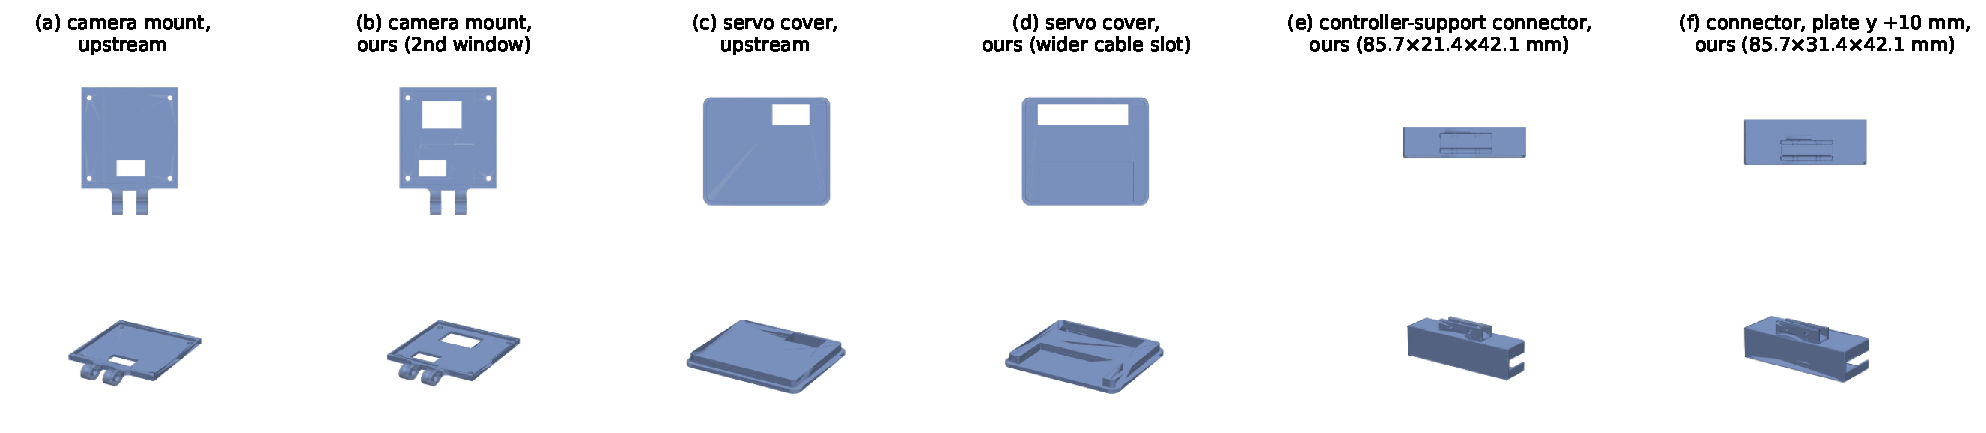
\includegraphics[width=\textwidth]{figures/fig10_handumi_mods.pdf}
\caption{업스트림 HandUMI 부품에 대한 우리의 수정(출력 메시 렌더링). (a,b) 카메라 마운트: 기존 창 위에 두 번째 창 추가. (c,d) 서보
컨트롤러 커버: 케이블 구멍 확장. (e) 업스트림 VR 컨트롤러 지지대를 대신하는 새 왼손 컨트롤러 지지대 커넥터. (f) 그 클램프 플레이트를
10\mm{} 늘린 현재 버전.}
\label{fig:hwmods}
\end{figure*}

\textbf{기록.} 에피소드 디렉터리에는 카메라별 MP4 하나, IMU 샘플(장치·호스트 타임스탬프), 그리퍼 샘플(랩·언랩 tick), 프레임별
메타데이터, 이벤트, 시계 앵커가 담긴 MCAP 파일, 그리고 메타데이터 파일이 들어 있으며, 닫힐 때에만 이름이 \code{.incomplete}에서
\code{.complete}로 바뀐다. 모든 스트림에는 호스트 단조 시계로 타임스탬프를 찍는다(IMU는 수신 시각, 그리퍼는 시리얼 트랜잭션의 중간
시점, 프레임은 캡처 시각).

\textbf{수집 프로토콜.} AUTO 루프(RESET $\to$ ARMING $\to$ HOLD $\to$ EPISODE $\to$ STOP)가 음성 신호와 함께 각 테이크를 진행한다.
ARMING은 정지 상태를 기다린다(0.25\,s 창에서 자이로 크기의 평균이 6\textdegree/s 미만, 가속도 크기의 표준편차가 0.35\,m/s$^2$ 미만,
최대 샘플 간격이 25\,ms 미만인 상태가 1\,s 동안 연속). 기록 시작 후의 정지 구간은 시각--관성 초기화 창 역할을 한다. 예비 QA(장치나
레코더 오류 없음, 빈 스트림 없음, 25\,fps 이상, 그리퍼가 20\,Hz 이상으로 샘플링되고 멈춰 있지 않으며 캘리브레이션 범위 안에 있고
범위의 5\% 이상 이동)를 통과한 테이크는 자동으로 보존된다.
\begin{itemize}
\item \emph{쌓기}: 50\mm{} 큐브 세 개(빨강, 파랑, 보라)를 고정된 접시 위에 지시문이 지정하는 여섯 순서 중 하나로 쌓는다. 예를 들어
``Stack the blue cube on the bottom, purple cube in the middle, and red cube on the top, on the plate.''이다. 테이크는 20\,s이며,
조작자가 손으로 큐브를 다시 놓는 10\,s의 리셋이 있다. 다음 순서는 가장 적게 수집된 순서(순서당 목표 50개)로 정해지므로, 순서는
무작위가 아니라 \emph{균형}을 맞춘 것이다. 배치는 수동 리셋을 통해 로봇 작업공간에 맞춘 기준 배치 주변에서 달라지지만 기록되지
않았으며, 에피소드별 배치 레이블은 없다.
\item \emph{로봇 유사}(HRL80): 실시간 피드백이 있는 30\,s 쌓기 테이크. 15\,Hz 격자에서 손목 각속도와 각가속도를 로봇 원격조작 데이터의
95번째 백분위수(0.996\,rad/s, 4.413\,rad/s$^2$)와 비교하며, 이를 넘는 틱이 10\% 초과이거나 파지가 두 번 미만이면 테이크를 검토한다.
\item \emph{접근}(HRA\_red): 오른손만, ``approach the red cube'', 10\,s 테이크.
\item \emph{원점이 있는 접근}(HRA\_A100): 위와 같되, 각 테이크는 로봇과 공유하는 테이프 원점 위에 조 끝을 대고 시작한다
(\ref{sec:res3}절).
\end{itemize}

\textbf{데이터셋.} 표~\ref{tab:data}에 본 보고서에서 사용한 모든 인간 및 로봇 데이터셋을 정리하였다. 인간 데이터는 모두 조작자 한 명이
기록하였다. 쌓기 에피소드 349개는 사흘(2026년 9월 15--17일)에 걸친 15개 세션에서 나왔으며, 총 2.20\,h(에피소드 중앙값 23.05\,s)이다.
순서별로 RBP 64, RPB 62, BRP 61, BPR 56, PRB 55, PBR 51이다. 초기 열 개 세션의 에피소드(55개)는 그리퍼 앵커를 사후에 도출했기 때문에
주 데이터 294개와 별도의 출처 도메인(``early'')으로 관리한다. 필터링 후 두 도메인은 비슷하게 동작한다. 로봇 데이터는 모두 reBot
B601에서 같은 여섯 순서 쌓기 과제를 원격조작한 시연이다.

\begin{table}[t]
\centering\footnotesize\setlength{\tabcolsep}{3pt}
\caption{데이터셋. 인간 데이터는 HandUMI로 기록하였고, 로봇 데이터는 같은 쌓기 과제의 reBot B601 원격조작 에피소드이다.}
\label{tab:data}
\begin{tabular}{@{}lp{56mm}@{}}
\toprule
이름 & 내용 \\
\midrule
Stacking & 양팔 에피소드 349개, 균형 6순서, 15 세션, 9월 15--17일 \\
HRL80 & 로봇 유사 쌓기 에피소드 60개(순서당 10개), 세션 하나 \\
HRA\_red & 오른손 접근 테이크 200개, 10월 3일 \\
HRA\_A100 & 테이프 원점이 있는 접근 테이크 107개, 10월 6일; 10월 7일에 27개 추가 \\
\midrule
R150 / R90 & 로봇 에피소드 150 / 90개(Gen-1 파인튜닝) \\
R312c & 로봇 에피소드 312개, 프레임 174{,}012개(Gen-2 파인튜닝) \\
R30 & R312c의 에피소드 150--179, 프레임 17{,}600개, 순서당 5개 \\
R384 & 로봇 에피소드 384개(scratch Gen-2 실행) \\
\bottomrule
\end{tabular}
\end{table}

\section{캘리브레이션}\label{sec:cal}
\textbf{손목 카메라.} 전체 해상도에서 Kannala--Brandt(등거리) 어안 모델을 사용하며, 25\mm{} 정사각형의 8$\times$5 체커보드로 Kalibr로
피팅한다(왼쪽 $f_x{=}789$, 오른쪽 $f_x{=}791$\,px). \textbf{카메라--IMU.} Kalibr~\cite{furgale2013kalibr} 결과 시간 오프셋은 30.2,
32.8\,ms, 평균 재투영 오차는 6.0, 5.6\,px로 높은 편이며, 이것이 자세 정확도를 별도로 검증하는 이유 중 하나다(\ref{sec:pose}절).

\textbf{카메라에서 TCP로.} TCP는 집게 중심이며, $x$는 접근 방향, $y$는 조가 닫히는 방향, $z=x\times y$이다. 회전은 고정된 축 순열
($x_\text{TCP}=z_\text{cam}$, $y_\text{TCP}=-x_\text{cam}$, $z_\text{TCP}=-y_\text{cam}$)이고, 병진은 캘리퍼 측정값(앞으로 95\mm, 아래로
95\mm)을 IMU 중력으로 측정한 카메라 피치(20.7\textdegree)만큼 회전한 것으로, $t=[0, 55.3, 122.5]$\mm{}를 얻으며 큐브 기반 피팅과 약
1\mm{} 이내로 일치한다. UMI가 CAD 상수를 쓰는 방식을 따라, 이 값은 장치 하나에서 측정하여 양쪽에 적용하였다.

\textbf{그리퍼 폭.} 각 프레임은 가장 가까운 그리퍼 샘플을 취한다. 기록된 정규화 값은 신뢰할 수 없었으므로(열린 끝이 기계적 정지점
너머에 있었고, 왼쪽 방향이 세션마다 뒤집혔다) Gen-1은 에피소드별 닫힘 앵커와 장치 범위(1136.6 / 1248.2 ticks)를 써서 raw tick으로부터
폭을 다시 계산하며, 폭 $=\mathrm{clip}(f,0,1)\times 67.5$\mm{}이다(개구 $67.5\pm5$\mm, 50\mm{} 큐브 파지 영상으로 추정). Gen-2는 이후의
캘리퍼 캘리브레이션(gcal1)을 사용한다. 0/20/40/60/80\mm{}에 구간별 선형 보간점을 두고 $g=\mathrm{clip}(w/80\,\text{mm},0,1)$로
정규화하며, 0 = 닫힘이다.

\textbf{시계와 동기화.} USB 지연은 항상 지연을 더하기만 하므로, IMU 장치 시각을 최소제곱 기울기로 호스트 시각에 대응시키고 절편은
잔차의 5번째 백분위수에 다시 고정한다. 그다음 카메라--IMU 오프셋을 적용한다. 카메라는 조금씩 다른 속도(30.003--30.026\,Hz)로 자유
동작하므로 프레임은 가장 가까운 캡처 시각으로 짝짓는다. 양팔 데이터에서는 왼 손목이 마스터 시계이며, 두 손목 자세가 모두 유효하고
오른 손목과 헤드 프레임이 20\,ms 이내로 매칭되면 행이 유효하다.

\textbf{로봇 측}(단일 팔 작업). 로봇의 고정 헤드 C922(HRA\_red 때와 같은 카메라, 같은 위치)를 같은 체커보드로 캘리브레이션했고
(48프레임, RMS 1.05\,px, $f=728.7$\,px), 로봇 베이스에서의 카메라 자세는 오른쪽 조 끝으로 보드의 네 모서리를 터치하여 구했다(FK
위치와 보드 PnP의 Kabsch 정렬, 잔차 2--6\mm). 로봇 손목 카메라는 보드 뷰 13장으로 캘리브레이션하고(0.16\,px RMS, $f=651.4$\,px),
핸드-아이 변환은 네 가지 방법(Tsai--Lenz~\cite{tsai1989handeye} 포함)으로 풀었으며, 베이스 내 보드 자세에서 1--2\mm,
0.3\textdegree{} 이내로 일치한다. 카메라는 TCP보다 169.5\mm{} 뒤, 축에서 76\mm{} 벗어나 있으며, 광축은 TCP $x$축보다
33\textdegree{} 아래를 향한다.

\textbf{TCP는 조 끝단이 아니다.} IK 스택의 TCP는 TCP $x$축을 따라 실제 조 끝단보다 약 82\mm{} 앞에 있다(FK 점을 손목 영상에 투영하여
확인). 따라서 접촉은 URDF 손끝 박스(TCP 뒤 70--80\mm, $\pm$19.6\mm)로 모델링하며, 그 가장 낮은 모서리를 접촉으로 간주한다.

\section{손목 자세와 메트릭 스케일}\label{sec:pose}
\textbf{단안 자세.} UMI는 모든 시연을 장면당 하나의 ORB-SLAM3 지도에서 위치 추정한다. 본 데이터에서는 이 방법이 실패하였다. 장면
변경 전에 만든 지도는 재위치 추정(relocalization)에 실패했고, 아래 마커 벤치마크에서 위치 궤적의 방향이 자주 역전되었다(역전율 중앙값 0.24, 우리가 채택한 방법은 0.07). 우리는 MASt3R-SLAM~\cite{murai2025mast3rslam}
(공식 코드, 커밋 고정, 유일한 패치는 빌드 수정)을 핀홀 뷰로 왜곡 보정한 RGB 손목 영상에 대해 단일 스레드, 매 프레임, 고정 시드로
실행한다. 전역 최적화 후 모든 프레임을 최종 키프레임 기준으로 다시 표현한다.
\begin{equation}
T_{WC}(f) = T_{WK}^{\text{final}}(k)\,T_{WK}^{\text{track}}(k)^{-1}\,T_{WC}^{\text{track}}(f),
\end{equation}
이는 Sim(3) 사슬이다. 재위치 추정 중에 추적된 프레임은 이후 키프레임이 되지 않는 한 무효이다. 그림~\ref{fig:traj}에 전형적인 궤적을
보였다.

\begin{figure*}[t]
\centering
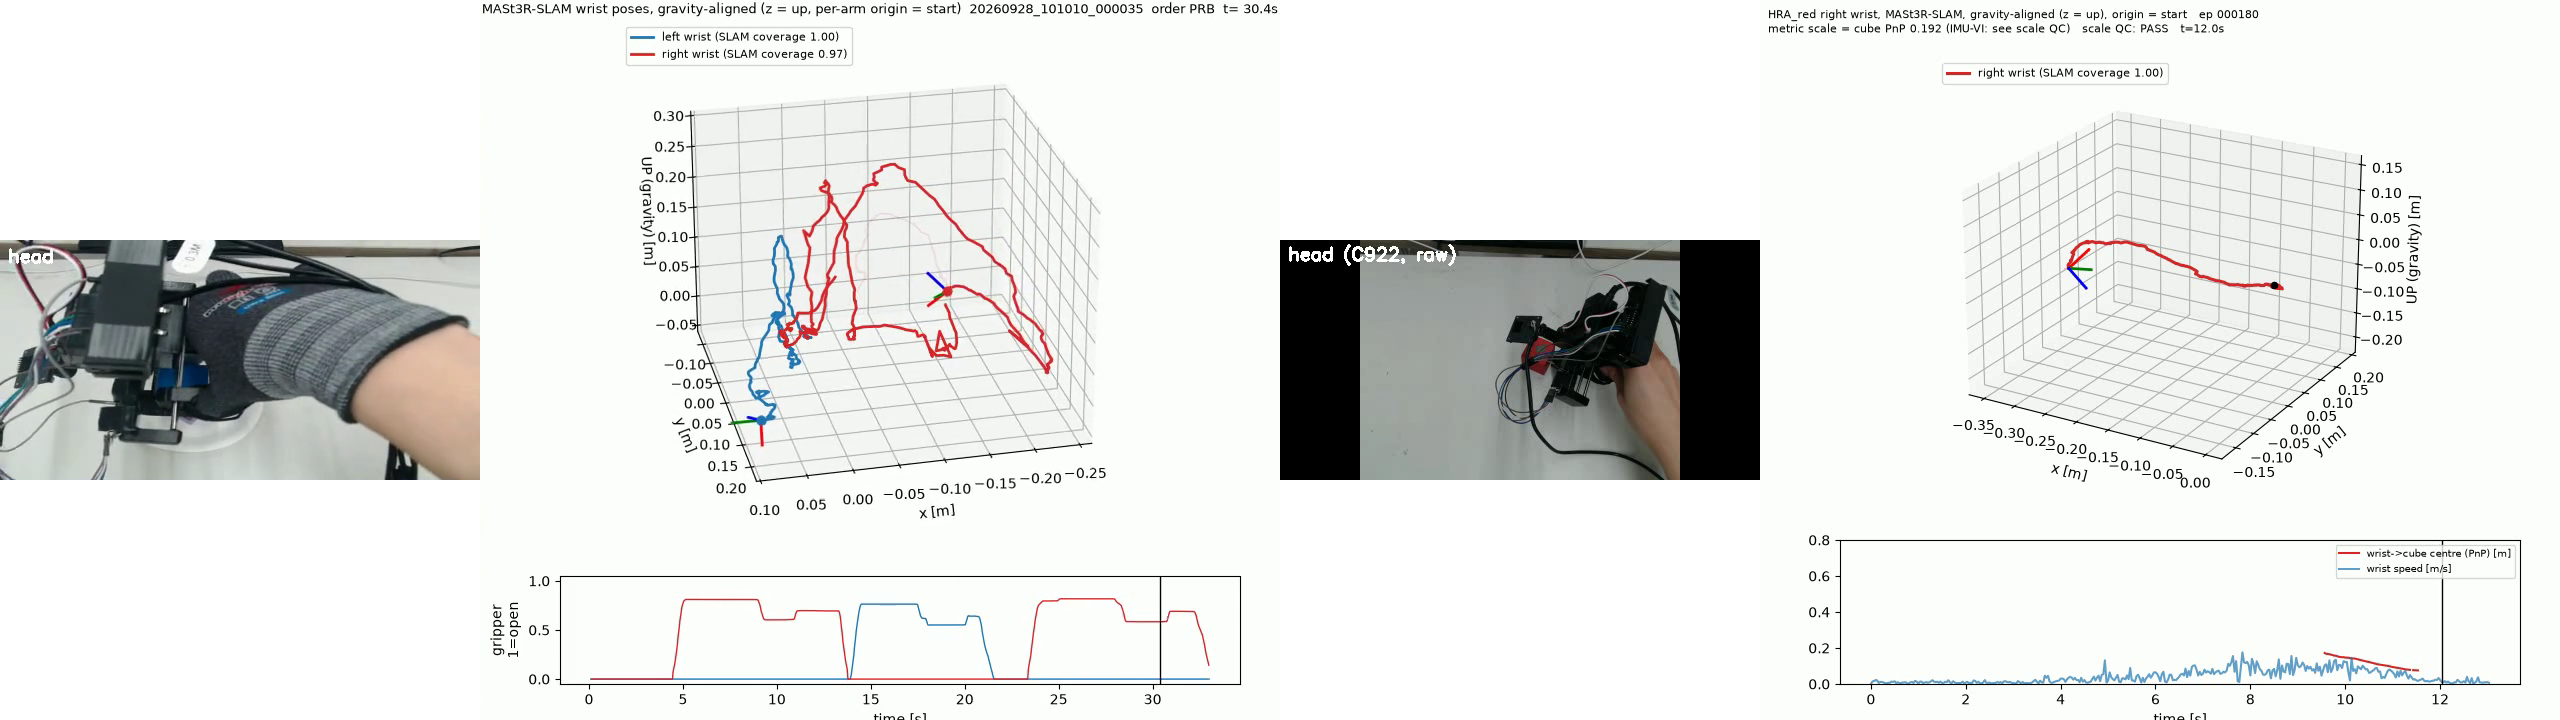
\includegraphics[width=0.8\textwidth]{figures/fig7_mast3r_trajectories.png}
\caption{HRL80 쌓기 테이크(순서 PRB)의 MASt3R-SLAM 손목 궤적. 왼쪽: 헤드 카메라와 두 손목 어안 카메라. 오른쪽: 중력 정렬(z 위쪽)된
궤적으로, 각 팔의 원점은 시작 자세이고 현재 공구 축을 표시(x 빨강, y 초록, z 파랑)하며 메트릭 스케일은 IMU에서 얻었다. 아래: 두
그리퍼(1 = 열림). 세 테이크(PRB, RBP, PBR)의 영상은 저장소의
\texttt{docs/media/mast3r\_trajectories/hrl80\_0000\{35,55,60\}\_wrist.mp4}에 있다.}
\label{fig:traj}
\end{figure*}

\textbf{스케일 1: IMU 시각--관성.} SLAM 궤적은 에피소드별 스케일 $s$를 제외하면 메트릭이다. $R_{wb}=R_{wc}R_{cb}$, 각 프레임 주위에서
박스 평균한 가속도계 샘플 $f_b$, 그리고 SLAM 카메라 위치와 $R_{wc}t_{cb}$의 Savitzky--Golay 이차 도함수(차수 3, 창 $W$)로 얻은 카메라
가속도 $a_\text{cam}$과 레버암 가속도 $a_\text{lever}$를 사용하면, 각 프레임은 다음 식의 세 행을 제공한다.
\begin{equation}
R_{wb}\,f_b - a_\text{lever} = s\,a_\text{cam} - g,
\end{equation}
이를 가장 긴 유효 구간에 대해 Huber 가중 반복 재가중 최소제곱으로 $s$와 $g\in\mathbb{R}^3$에 대해 푼다. 양변이 같은 필터를 거치므로
어떤 것도 두 번 적분하지 않는다. $s>0$이고 $|g|\in[8.81,10.81]$\,m/s$^2$이면 스케일이 유효하다.

\textbf{자세 벤치마크.} 80\mm{} ArUco 마커 네 개가 보이는 시연 14개(손 트랙 28개)를 데이터셋과 같은 GPU에서 실행하였다. 정답 스케일은
열 프레임 떨어진 프레임 쌍에서 마커 변위와 SLAM 변위의 비의 중앙값이다. 바이어스 없는 $W=15$를 시연 9개의 피팅 분할에서 선택하였다.
held-out 시연 5개(트랙 10개)에서 IMU 스케일을 적용한 MASt3R-SLAM은 추적 커버리지 중앙값 1.00(저장된 지도를 쓴 ORB-SLAM3는 0.03),
스케일 오차 p50/p90 4.6/17.0\%(단일 전역 상수는 18.5/23.8\%),
회전 오차 p50/p90 0.84/2.13\textdegree{}, UMI 방식 16스텝 상대 위치 오차 p90 11.3\mm{}를 보인다. 시연 자체에는 정답(ground truth)이
없다.

\textbf{스케일 2: 크기를 아는 큐브.} 느리고 부드러운 동작에서는 가속도계가 IMU 피팅을 거의 구속하지 못한다. HRA\_red 테이크 200개에서
IMU 스케일의 중앙값은 0.012이며, 그중 95개에서는 물리적으로 불가능한 0 또는 음수 값을 보인다(그림~\ref{fig:cube}b). 빨간 큐브(모서리
38\mm)는 정지해 있다. 큐브가 보이는 프레임에서 HSV로 큐브를 분할하고, 그 실루엣을 두 면 또는 세 면 모델로, 한 면이 정면에서
35\textdegree{} 이내로 보일 때는 단일 면 모델로 피팅한 뒤 PnP를 푼다. 큐브가 정지해 있으므로 그 중심 $c_i=p_i + k\,R_i t_i$는 일정해야
하며, 이로부터 역스케일을 닫힌 형태로 얻는다.
\begin{equation}
k = -\frac{\sum_i (p_i-\bar p)\cdot(u_i-\bar u)}{\sum_i\lVert u_i-\bar u\rVert^2},\qquad u_i=R_i t_i,\quad s=1/k,
\end{equation}
여기에 MAD 트리밍과 부트스트랩 재표본 200회를 적용한다. 테이크는 PnP 프레임 10개 이상, 부트스트랩 퍼짐 10\% 이하, 큐브 중심 잔차
2\,cm 이하를 만족해야 한다. IMU 스케일을 신뢰할 수 있는 HRL80 쌓기 테이크에서는 오른손 에피소드 57개 중 37개가 PnP 유효이며, PnP/IMU
비의 중앙값은 1.062(p16--p84 0.959--1.274; 그림~\ref{fig:cube}a)이다.

\begin{figure*}[t]
\centering
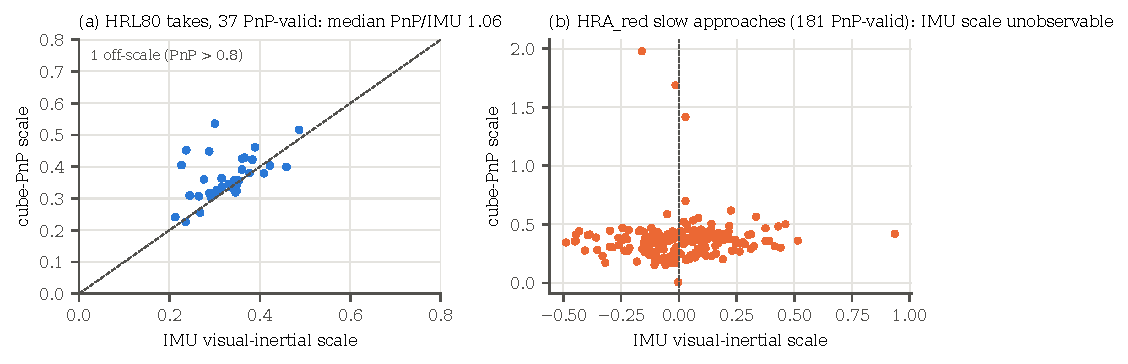
\includegraphics[width=\textwidth]{figures/fig6_cube_scale.pdf}
\caption{IMU와 큐브 PnP로 구한 MASt3R-SLAM 궤적의 에피소드별 메트릭 스케일. (a) IMU 스케일을 신뢰할 수 있는 HRL80 쌓기 테이크.
(b) HRA\_red 접근 테이크: IMU 스케일이 0 주변에 흩어진다.}
\label{fig:cube}
\end{figure*}

\textbf{스케일 3: 공유 원점에서의 테이블 평면.} HRA\_A100에서는 원점 홀드 동안 손끝이 플레이트에 닿아 있으므로, 첫 MASt3R 키프레임은
알려진 거리에서 테이블을 본다. 손가락을 제외하고 RANSAC으로 평면을 최대 세 개 피팅하며, 플레이트와 평행한 가장 큰 평면을 테이블로
택한다. $s=|n\cdot t_\text{tip}|/(s_0\,|d|)$이며, $t_\text{tip}$은 카메라 좌표계의 손끝, $s_0$는 키프레임의 Sim(3) 스케일이다.
40개 테이크에서 큐브 PnP 대비 비의 중앙값은 0.999, 에피소드별 오차는 p50 8\%, p90 37\%이다. 각 에피소드는 큐브 PnP가 유효하면 이를,
그렇지 않으면 평면을 사용하며(107개 중 각각 35개, 72개), IMU는 사용하지 않는다.

\textbf{드러나지 않는 자세 점프.} 에고와 로봇의 상태 통계를 비교한 결과, 로봇 데이터에는 없는 행당 100\mm{} 초과의 상태 점프가 에고
데이터에 있었다. 두 원인이 섞여 있었다. 첫째, 내보낸 데이터셋에는 학습 행만 있으므로 ``인접'' 프레임이 수 초 떨어져 있을 수 있다.
30\mm{}를 넘는 겉보기 점프 2{,}598개 중 1{,}482개(57\%)가 이런 시간 공백이며, 인접 여부는 행 타임스탬프로 판단해야 한다. 둘째, 나머지
점프는 실제이다. MASt3R-SLAM은 추적 손실을 표시하지 않은 채 30\,Hz 한 프레임 안에서 카메라를 10\,cm 이상 옮기는 경우가 가끔 있다(학습
에피소드 24개에서 3\,m/s보다 빠른 원시 스텝 55개, 그 어느 것도 앞서 손실 플래그가 없었다). 필터는 66.7\,ms 행당 100\mm{} 또는
45\textdegree{}를 넘는 스텝, 또는 0.3\,m/s보다 느린 두 스텝 사이에 고립된 50\mm{} 초과 스텝에 플래그를 단다. 자세가 되돌아오면
이벤트는 스파이크이며 해당 샘플만 무효화한다. 그렇지 않으면 단방향 점프로 보고 그 팔 트랙의 나머지를 버린다. 시작점에 고정된 상태가
그 이후로 틀리게 되기 때문이다.

\textbf{카메라--IMU 일관성.} 자이로와 SLAM 각속도가 일치하지 않는 세션(다른 곳의 0.92--0.98 대비 코사인 중앙값이 0 근처)은 격리한다.
접근 데이터에서는 오른 손목의 내보낸 카메라--IMU 회전이 카메라 $x$축에 대해 약 18\textdegree{} 틀려 있었음이 드러났다(수정 후 큐브
축 오차 17.8$\to$3.4\textdegree). 수정 전에 계산한 IMU 기울기 통계는 최대 그만큼 틀려 있으며, 스케일을 큐브 PnP에서 얻은 학습 자세는
영향을 받지 않았다.

\section{인간 동작을 로봇 데이터로 변환}\label{sec:conv}
\subsection{1세대: 관절 공간 리타게팅}
\textbf{세그먼트와 게이트.} 동기화된 유효 행을 겹치지 않는 65프레임 세그먼트(2.17\,s)로 자른다. 팔별로 세그먼트는 유효한 메트릭
스케일을 가져야 하고, 행의 95\% 이상이 로봇 작업공간 안에 있어야 하며(목표는 로봇 원격조작 TCP 자세 6{,}000개 중 최근접 이웃이
50\mm{} 이내이고 방향 차이가 20\textdegree{} 이내이면 내부로 본다), 모든 행에서 IK 해가 있어야 한다. 두 팔이 모두 통과하면 세그먼트는
양팔 세그먼트이다. 각 TCP 궤적은 URDF 기반 최소제곱 IK로 reBot B601 6-DoF 팔에 매핑된다. 절대적인 작업공간 기하는 에피소드 간에
복원할 수 없으므로, 각 세그먼트를 고정된 로봇 시작 자세(로봇 원격조작 데이터의 활동 자세 중앙값)에 다시 앵커링한다. 즉 동작은
전이되지만 큐브의 절대 위치는 전이되지 않는다. 조 인코더 값은 이진 그리퍼 명령이 된다.

\textbf{퍼널.} 표~\ref{tab:funnel}에 각 게이트가 제거하는 것을 정리하였다. 65개 에피소드가 65프레임 전체 윈도에 대한 $\le$20\,ms
동기화 요건을 통과하지 못한다. 나머지 284개에서 양팔 후보 세그먼트 1{,}306개가 나오며, 그중 677개는 로봇 작업공간을 벗어나고, 50개는
메트릭 스케일 검사에, 18개는 IK에 실패하여 561개(43.0\%)가 남는다. 두 세션(에피소드 6개)은 IMU--카메라 회전 불일치로 격리되었으며
세그먼트를 하나도 기여하지 않았다. 세그먼트의 47\%가 에피소드 첫 5\,s 안에서 시작한다.

\textbf{분할.} 양팔 세그먼트가 하나 이상인 259개 에피소드를 에피소드 단위로 무작위 분할(seed 0, 10\%)하여 학습 233 / 검증 26, 즉
세그먼트 504/57개, 프레임 32{,}760/3{,}705개로 나눈다. 양쪽에 걸친 에피소드는 없다. 분할은 층화되지 않았으며, 검증 세트는 순서당 3--6
에피소드, main 22 / early 4개이고, 격리되지 않은 13개 세션 중 9개에서 왔다.

\begin{table}[t]
\centering\footnotesize
\caption{쌓기 에피소드 349개에 대한 Gen-1 처리 퍼널(저장소의 집계 파일로부터 재계산한 수치).}
\label{tab:funnel}
\setlength{\tabcolsep}{4pt}\begin{tabular}{@{}lrr@{}}
\toprule
단계 & 에피소드 & 세그먼트 \\
\midrule
기록됨(KEEP) & 349 & -- \\
자세 + 그리퍼 내보내기(궤적 698개) & 349 & -- \\
동기화 $\le$20\,ms, $\ge$65프레임 윈도 & 284 & 1{,}306 \\
\quad $-$ 작업공간 / 메트릭 스케일 / IK & & $-$677 / $-$50 / $-$18 \\
양팔 세그먼트 $\ge$1개(학습 풀) & 259 & 561 \\
\quad 학습 / 검증(에피소드 단위, seed 0) & 233 / 26 & 504 / 57 \\
\bottomrule
\end{tabular}
\end{table}

\textbf{리타게팅 v2.} 단일 시작 앵커가 주된 손실 원인이었다. 모든 세그먼트가 하나의 로봇 자세에서 시작했기 때문에 대부분이 작업공간을
벗어났고, 리타게팅된 궤적은 하나의 자세 클러스터만을 덮었다. v2는 이를 엄격한 예산 아래의 다중 시드 리타게팅으로 대체한다. 모든 실제
로봇 수치(시드 뱅크, 작업공간 게이트, 자세 페널티, 궤적 윈도)는 로봇 에피소드 30개에서만 가져오고, 결과는 이와 겹치지 않는 로봇
에피소드 120개에 대해 측정한다. $2^{17}$개 Sobol 샘플로 된 시드 뱅크를 작업공간, 테이블 바닥, 조작성, 팔 간 간격($\ge$75\mm)으로
걸러 시드 1{,}195개를 남긴다. 변형 K는 위치, 회전, 관절 속도, 관절 가속도에 대한 비용 아래 상위 시드 8개를 롤아웃하고, Kr은 로봇
데이터까지의 자세 거리를 추가하며, 궤적 윈도 검색(TR)은 각 인간 세그먼트를 가장 가까운 실현 가능한 로봇 궤적 윈도(96-D 상대 동작
특징 기준 최근접 64개)에서 시작한다. 표~\ref{tab:retarget}는 같은 후보 세그먼트 1{,}229개에서 이들을 비교한다. TR이 가장 로봇에
가깝다. held-out 로봇 데이터까지의 자세 거리가 1.49에서 0.27\,rad(중앙값)로 줄고, 시작 자세는 1개가 아닌 100개 클러스터에 걸친다.
TR은 빠른 동작을 배치하지 못하므로 기구학 변형보다 해결하는 세그먼트가 적다. TR과 Kr이 모두 해결하는 686개 세그먼트에서 두 방법의
관절 속도 분포는 비슷하므로(W1 0.00207 대 0.00226), TR이 더하는 것은 동역학 개선이 아니라 자세 개선이다. 남은 실패는 거의 모두
``작업공간과 호환되는 윈도 없음''이다(미해결 402개 중 399개).

\begin{table}[t]
\centering\footnotesize\setlength{\tabcolsep}{3.5pt}
\caption{259개 에피소드의 후보 세그먼트 1{,}229개에 대한 리타게팅 변형 비교, held-out 로봇 에피소드 120개 기준.
NN: 로봇 자세까지의 최근접 이웃 관절 공간 거리(rad, p50/p90). W1: 스텝당 $|\Delta q|$의 Wasserstein 거리.}
\label{tab:retarget}
\begin{tabular}{@{}lcccc@{}}
\toprule
변형 & 사용 가능 & NN p50 / p90 & 시작 클러스터 & W1 $|\Delta q|$ \\
\midrule
v1 단일 앵커 & 36.5\% & 1.49 / 1.55 & 1 & 0.00197 \\
v2-K 다중 시드 IK & 66.6\% & 1.21 / 1.60 & -- & 0.00275 \\
v2-Kr + 자세 페널티 & 67.0\% & 0.44 / 0.74 & -- & 0.00310 \\
v2-TR 윈도 검색 & 56.1\% & 0.27 / 0.45 & 100 & 0.00208 \\
\bottomrule
\end{tabular}
\end{table}

\textbf{로봇 유사 재수집.} 손실이 수집 방식의 문제인지 검증하기 위해 로봇 유사 프로토콜로 HRL80(에피소드 60개, 순서당 10개)을
기록하였다. 해석 규칙은 리타게팅 전에 고정하였다. 실시간 회전 속도는 절반으로 줄었으나(임계값 초과 비율 중앙값 0.144에서 0.067),
에피소드별 TR 수율은 변하지 않았고(0.59 대 0.59) TR 사용 가능 비율은 56.1\%에서 58.9\%로 오르는 데 그쳤다. 실시간 로봇 유사도와 TR
수율의 에피소드별 상관은 약하다(Spearman $\rho=-0.11$, $p=0.05$, 통합 $n=316$). 수집 방식이 아니라 작업공간 배치가 여전히 주된 실패
원인이다. 최종 TR 데이터셋은 두 수집분을 합친 것으로, 원본 에피소드 316개에서 나온 세그먼트 996개(학습 896 / 검증 100)이며 원래의
세그먼트 689개는 비트 단위로 동일하게 보존된다.

\subsection{2세대: 데카르트 계약(CART20)}
로봇 관절로의 리타게팅에는 두 가지 비용이 있었다. 작업공간 및 IK 게이트가 후보 동작의 삼분의 일에서 절반을 제거했고, 관절 공간 목표가
로봇 정책을 파인튜닝하는 데카르트 액션 공간과 달랐다. Gen-2는 각 인간 손목 궤적을 로봇 원격조작 데이터와 같은 상대 엔드이펙터
표현으로 직접 변환하여, 에고 샘플과 로봇 샘플이 하나의 텐서 계약을 공유하도록 한다.

\textbf{계약.} 행은 15\,Hz로 저장한다. 행 시각 $t$와 각 팔에 대해 액션은 미래 자세 16개의 청크
\begin{equation}
A_k = T(t)^{-1}\,T(t+k\Delta),\qquad k=1,\dots,16,
\end{equation}
이며, $\Delta = 50.05$\,ms(로봇 데이터의 스텝, 합계 0.80\,s)이다. 순차가 아니라 현재 시점에 고정되고, 원시 30\,Hz 궤적에서
보간한다(위치는 선형, 회전은 SLERP, 50\,ms 이내로 떨어진 유효 샘플 사이에서만). 각 팔은 위치, 6-D 회전, 그리퍼 값을 제공하며(두 팔
합계 20차원, ``CART20''), 모델의 32-D 액션은 정확히 0이고 지도되지 않는 12개 차원으로 패딩된다. 상태는 각 팔의 자기 과제 시작 자세에
대한 상대 자세 $T(t_0)^{-1}T(t)$와 그리퍼 값 두 개로, 로봇 상태와 같은 배치이다(좌우가 공유하는 SLAM 프레임은 없다). 그리퍼는 조
개구를 80\mm{}로 나눈 값이며, 관측된 최댓값이 0.847이므로 ``완전 열림''에는 도달하지 않는다. 행은 $t$에서 두 팔이 모두 유효하고, 16개
목표가 모두 유효하며, 20\,ms 이내에 헤드 카메라 프레임이 있을 때만 남긴다. 패딩은 없으며 작업공간이나 IK에 의한 선별도 없다. 합성
테스트 열한 개가 계약을 고정한다.

\textbf{데이터.} 원천은 손별 IMU 스케일이 유효한 원래 쌓기 에피소드 273개와 HRL80 에피소드 60개이며, 그중 3개는 한 손의 IMU 스케일이
유효하지 않아 제외되어 330개가 남는다. 행 111{,}533개 중 57{,}283개(51.4\%)가 사용 가능하며, 나머지는 추적 손실, 동기화 공백, 또는
에피소드의 마지막 0.8\,s에 걸린다. 분할은 Gen-1에서 고정한 것을 쓴다(검증 = held-out 에피소드 26개와 HRL80 에피소드 49--54). 학습
에피소드 298개에 행 51{,}612개, 검증 에피소드 32개에 행 5{,}671개이다. 자세 점프 필터(\ref{sec:pose}절)는 학습 에피소드 42개의 이벤트
44건에 작용하며 에피소드 하나를 통째로 제거한다. 학습은 에피소드 297개, 행 48{,}411개($-6.20$\%)로 줄고 검증은 변하지 않는다. 시간상
인접한 행 사이의 최대 스텝은 422.5에서 90.5\mm{}로, 100\mm{} 초과 스텝은 18개에서 0개로 줄며, 3\,m/s보다 빠른 원시 스텝 7개는 유효 행
안에 남는다.

\textbf{에고 데이터와 로봇 데이터의 차이.} 에고 에피소드 60개와 로봇 에피소드 60개에서, 에고 자세를 로봇 시작 자세에 붙였을 때 로봇
IK는 에고 위치의 99.7\%(왼쪽)와 99.5\%(오른쪽), 에고 전체 자세의 72.3\%/74.6\%에 도달한다. 로봇에서 쓰는 IK 구성은 손목 관절 하나를
잠그므로 로봇 \emph{자신의} 기록 자세도 45.2\%/52.2\%만 재현하는데, 이는 인간 데이터와 무관하게 존재하는 배포상의 한계이다. 에고 손은
더 작은 작업공간을 쓰고(상태 p95 0.221/0.214\,m 대 0.395/0.369\,m), 0.4\,s 이동량은 비슷하며(p95 93/99 대 91/100\mm), 에고는 두 손이
동시에 정지해 있는 경우가 훨씬 잦다(샘플의 19.5\% 대 2.4\%). 가장 큰 차이는 시각적이다. 선명도 척도인 이미지 Laplacian의 분산 중앙값이
에고 손목 어안 시점에서는 1{,}854/1{,}487, 로봇 손목 카메라에서는 59/64이다.

\textbf{로봇 유사 손목 렌더링.} 시각적 격차를 줄이기 위해 어안 프레임을 같은 방향의 가상 핀홀 카메라로 다시 렌더링할 수 있으며,
따라서 레이블은 그대로 유효하다. 수평 화각은 62--70\textdegree{}이고, 로봇처럼 조가 아래쪽에 오도록 주점을 아래로 옮긴 뒤 축소,
블러, JPEG 압축, 광도 지터를 적용한다. ROBOT100은 이를 모든 프레임에 적용한다.

\subsection{단일 팔 변형과 공유 작업 좌표계}
\textbf{오른팔 전용 계약.} 텐서 레이아웃은 바뀌지 않는다. 왼쪽 상태는 그리퍼 0인 항등 자세, 왼쪽 액션은 0 동작이며, 20-D loss mask가
오른팔의 위치와 회전(9차원; 조는 사용하지 않음)만 지도한다. 작업 문자열은 ``Approach to the red cube''이다.

\textbf{로봇 카메라 렌더링(robotcam v2).} 첫 버전(v1)은 위의 추정한 카메라로 손목 뷰를 렌더링했다. 실측한 로봇 C922는 수평 화각이
52\textdegree{}이고 주점이 중앙에 있으므로, v1은 로봇 카메라보다 접근 과정에서 훨씬 늦게 큐브를 보여 주었다. v2에서는 로봇 카메라의
각 픽셀 광선을 어안 모델에 투영하여 재표본하고, 레이블을 핸드-아이 변환을 통해 로봇 TCP 자세로 표현한다(로봇 TCP $\to$ UMI TCP: $y$축에
대해 $-33$\textdegree, $t=(-94.8, 2.4, 38.4)$\mm).

\textbf{작업 좌표계 G.} 로봇 그리퍼에서 약 35\,cm 떨어진 헤드 카메라 베이스 플레이트 위의 테이프 십자 표시가 작업 원점이다. 로봇
오른쪽 조 끝단으로 테이프 선 위의 세 점을 터치했다. 세 점은 60.4\mm{} 기준선에서 0.38\mm{} 이내로 공선이며, 높이는 2\mm{} 이내로
일치한다. G의 원점은 십자 중심이고, $x$축은 테이프를 따라 인간 쪽을 향하며, $z$축은 베이스 $z$축과 같다. 로봇 베이스에서 원점은
$(59.0, -74.9, 6.2)$\mm, 방위각은 47.09\textdegree{}이다. 35\mm{} 플레이트를 고려하면 테이블은 $z=-27.1$\mm{}에 있다. 인간 측에서
원점 자세는 원점 홀드 동안의 위치 중앙값과 평균 회전이다. 그 yaw는 테이크마다 십자 주변의 테이블 특징을 기준 테이크와 매칭하여
측정하고(오차 p50 0.21\textdegree, p90 1.17\textdegree), 기울기는 IMU 중력에서 얻는다. 평균 yaw를 가정했을 때는 잘못된 기각과
57\mm{}의 끝점 높이 퍼짐이 발생했다(측정 yaw 사용 시 35\mm). 홀드 자체의 반복성은 14\mm(p50; p90 37\mm), 6.2\textdegree(p50)이며,
이때 카메라는 63.7\textdegree{} 아래로 기울어져 있다.

\textbf{테이블 인지 변환.} 인간의 동작을 G에서 표현하고 로봇 시작 자세에서 출발시키면 손끝이 테이블 속으로 들어갈 수 있다. 따라서
궤적을 자신의 시작점에서 로봇 시작 자세 쪽으로, 테이크 동안 0으로 감쇠하는 smoothstep 가중치로 변형한다. 수평 위치, 높이, 회전에는
각기 다른 스케줄을 쓰므로 큐브 근처의 인간 끝점은 유지된다. 그다음 높이 보정 $c$를 테이크마다 이차 계획 문제로 푼다.
\begin{equation}
\begin{aligned}
\min_c\;& \textstyle\sum c^2+50(\Delta c)^2+2000(\Delta^2 c)^2+60\,m\,(c-g)^2\\
\text{s.t.}\;& z_\text{tip}+c\ge z_\text{table}+5\,\text{mm},
\end{aligned}
\end{equation}
여기서 $c_0=0$, 끝점 들어올림은 최대 30\mm{}이며, $g$는 낮은 프레임을 12\mm{} 여유 쪽으로 끌어올린다. 결과는 IK로 재생한다. 테이크는
PASS(들어올림 $\le$20\mm), PASS-CORRECTED(20--30\mm), 또는 기각(IK 성공률 98\% 미만, 원점 홀드 또는 yaw 누락, 홀드 중 10\mm{} 넘게
이동)으로 분류한다. 표~\ref{tab:ct}에 변형들을 정리했다. CT4는 위치, 높이, 회전을 각기 다른 스케줄로 감쇠한다. CT5는 측정된 원점 yaw,
보정된 IMU 중력, G에서의 절대 상태, 홀드 게이트를 추가한다. CT6는 로봇 시작 자세를 6\,cm 뒤, 4\,cm 아래로 옮긴다. CT5와 CT6는 손끝
여유 p50 12.6\mm, 최소 7.6\mm{}로 86개 테이크를 유지한다. 기각의 대부분은 첫 세션(원점 홀드 도입 이전)이거나 원점 yaw를 측정할 수
없었던 테이크이다.

\begin{table}[t]
\centering\footnotesize\setlength{\tabcolsep}{3pt}
\caption{HRA\_A100의 테이블 인지 변환. 채택 = PASS + PASS-CORRECTED. 여유: 보정 후 테이블 위 손끝 높이(채택된 테이크 기준).}
\label{tab:ct}
\resizebox{\columnwidth}{!}{\begin{tabular}{@{}lcccc@{}}
\toprule
변형 & 테이크 & 채택 & 주요 기각 사유 & 여유 p50 / 최소 \\
\midrule
C (평균 yaw) & 107 & 81 & 들어올림 $>$30\,mm 10, 이전 세션 7 & 19.5 / 7.0\mm \\
CT4 (축별 감쇠) & 107 & 87 & 들어올림 10, 이전 세션 7 & 20.6 / 7.9\mm \\
CT5 (yaw, G, 홀드 게이트) & 107 & 86 & yaw 미측정 9, 이전 세션 7 & 12.6 / 7.6\mm \\
CT6 (시작점 뒤/아래) & 107 & 86 & CT5와 동일 & 12.6 / 7.6\mm \\
CT7 (낮은 시작점, +27) & 134 & 90 & IK 19, yaw 11, 이전 세션 7 & 12.4 / 7.6\mm \\
\bottomrule
\end{tabular}}
\end{table}

\section{모델 및 학습}\label{sec:model}
\textbf{모델.} 공개 \texttt{xvla-base} 체크포인트에서 LeRobot~\cite{cadene2024lerobot}을 통한 X-VLA~\cite{zheng2025xvla}를 사용한다.
Florence-2~\cite{xiao2024florence2} vision-language 인코더, 24층 soft prompt 트랜스포머(hidden 1024, 헤드 16개),
flow matching~\cite{lipman2023flow} 액션 헤드로 구성되며, 파라미터 879M개가 모두 학습 대상이다. 입력은 세 시점(헤드, 왼손목,
오른손목; 224\,px로 리사이즈), 지시문, 고유수용 상태이다. 학습에서는 $t$를 뽑아 $x_t=\varepsilon t+a(1-t)$를 만들고 깨끗한 액션을
회귀하며, 추론은 노이즈에서 시작하여 기본 10스텝으로 적분한다. Gen-2를 위해 공개 헤드(20-D 액션과 상태)를 32-D 액션과 20-D 상태로
넓혔다. 기존 행은 그대로 복사하고, 확장된 모델이 base 모델을 재현하는지 확인하였다.

\textbf{어떤 soft prompt인가?} X-VLA는 soft prompt 32개로 이루어진 30개 집합 중 하나와 도메인별 상태/액션 프로젝션을 선택하는
데이터셋/embodiment id를 조건으로 받는다. 첫 실행들은 id~0을 썼다. 공개 base 가중치를 읽어 보면 슬롯 10--17만 학습된 적이 있다.
나머지 22개 슬롯에서는 인코더와 디코더 bias가 정확히 0이고 프롬프트 가중치가 초기값 근처에 머문다. 따라서 본 연구에서 쓴 id 0과 6은
모두 학습되지 않은 슬롯이었다. 학습된 슬롯이 더 나은 출발점인 것도 아니다. R312c에서의 초기 손실은 슬롯 0이 1.11, 6이 1.12, 15가
1.61, 10이 2.35, 16이 2.65, 17이 4.07, 11이 22.80이다. 모든 Gen-2 실행은 사용되지 않은 슬롯 20을 본 embodiment 전용 슬롯으로 쓴다.

\textbf{Gen-1 레시피.} 상태 시각 $t$에 대해 모델은 리타게팅된 의사 관절의 누적 관절 변위로 이루어진 30스텝 청크
$a_i = q_{t+5+i}-q_t$, $i=0,\dots,29$를 예측하며(5프레임 선행, 따라서 청크는 0.2--1.17\,s 앞을 덮는다), 여기에 절대 그리퍼를 더한다.
상태는 14-D(팔마다 관절각 6개와 이진 그리퍼)이다. 두 보조 항이 관절 공간을 측정된 인간 동작에 묶는다. (C) 측정 궤적의 상대 TCP
위치를 남는 액션 차원에서 예측하는 항(가중치 2.0)과, (D) $\mathrm{FK}(q_t+\hat a_i)$와 측정 TCP 위치 사이의 순기구학 손실(가중치
20)이다. 목표는 측정된 인간 전이이며, 로봇 명령으로 다시 레이블링한 값은 절대 쓰지 않는다. 최적화: 300k 스텝, 배치 4, AdamW(lr
$10^{-4}$, vision-language 그룹은 0.1$\times$, weight decay $10^{-4}$, warm-up 1k, $2.5\times10^{-6}$까지 cosine decay), gradient
clipping 10, fp32, RTX~4090 한 대, 10k마다 체크포인트. 체크포인트 선택 규칙(최소 geo score, \ref{sec:eval}절)은 학습 전에 고정하였다.

\textbf{Gen-2 레시피.} 손실은 액션 차원 0--19에 대한 MSE이며, 차원 20--31은 학습과 추론 모두에서 모든 디노이징 스텝마다
트랜스포머의 입력과 출력에서 0으로 둔다. 사전 점검(preflight)은 패딩 목표가 무시되고 패딩 그래디언트가 사라지는지를 확인한다. 배치 8,
8-bit AdamW(정책 학습률 $10^{-4}$, warm-up 1k, 정확히 마지막 스텝에서 끝나는 cosine decay), bf16 혼합 정밀도, seed 1000. 단일 팔
데이터에서는 마스킹된 목표를 뺄셈 전에 detach한 예측으로 대체하고, 손실을 지도되는 원소 수로 정규화한다. 300스텝 스모크 테스트로
마스킹·패딩된 차원이 정확히 0의 그래디언트를 받는 것을 확인하였다. 파인튜닝은 새 옵티마이저로 시작하며 로봇 데이터셋의 정규화 통계를
쓴다. 공동 학습은 배치마다 정확히 에고 샘플 네 개와 로봇 샘플 네 개를 뽑는다.

\textbf{운영.} 작업은 RTX~4090 또는 RTX~5090 노드에 고정한 Ray 클러스터에서 실행한다(두 노드의 PyTorch 버전이 달라 노드 간 실행은
비트 단위로 같지 않다). 런처는 사용 중인 GPU, 코드 해시나 도메인 id 불일치, 그리퍼 계약 게이트 실패, 디스크 공간 부족 시 시작을
거부한다. 각 본 실행 전에 저장·재개를 포함한 짧은 스모크 실행을 하며, 아카이버는 모든 체크포인트를 SHA-256 검증과 함께 외부 저장소로
복사한 뒤 노드에서 삭제한다.

\section{평가 프로토콜}\label{sec:eval}
\textbf{Gen-1 오프라인.} held-out 에피소드 26개에서 검증 세그먼트 57개 각각의 시작 프레임 7개(0--30 구간에서 5프레임 간격)를 취해
샘플 399개, 팔-샘플 798개를 만들고, 예측 청크를 기록된 미래와 비교한다. 예측 구간 $k\in\{1,4,8,16,30\}$에 대해
$\mathrm{FK}(q_t+\hat a_k)$와 측정 TCP 사이의 TCP 위치 오차(중앙값, mm), 관절 MAE와 \emph{무동작} 예측기($\hat a\equiv0$)의 관절
MAE, 예측·측정 TCP 변위 사이의 코사인을 보고한다. \emph{geo score}는 다섯 예측 구간에 대한 TCP 오차 중앙값의 평균이다. 대부분의
샘플이 거의 정지 상태이므로, 모든 지표를 \emph{동작} 부분집합, 즉 $k{=}30$까지 측정 TCP가 $\ge$20\mm{} 움직이는 팔-샘플(798개 중
187개, 23.4\%)에 대해서도 보고한다. 이 게이트는 60k 체크포인트를 평가한 뒤에 추가되었으며 보고용으로만 쓴다.

\textbf{Prompt swap.} 지시문 사용 여부를 검증하기 위해 최종 체크포인트에 모든 샘플을 여섯 순서 지시문 각각으로 같은 노이즈 시드를
써서 질의하고, 올바른 지시문으로는 두 개의 추가 시드에서도 질의한다. 여섯 예측의 퍼짐은 지시문의 효과를, 시드 간 퍼짐은 샘플링
노이즈 하한을 나타낸다. \textbf{대응 부트스트랩(paired bootstrap)}: 두 초기값 사이의 geo score 상대 차이를 에피소드 수준
재표본(10k회, 두 모델에 동일)으로 추정한다.

\textbf{Gen-2 진단.} 로봇 프레임에서의 teacher-forced 방향 코사인(동작 프레임에 대해 $k$=4/8/16에서 예측 대 기록 병진)을 모든 좌우
교환과 축 부호 반전에 대해 반복한다. 이미지/상태 도메인 교환, 규약 검사로서 손목 영상의 광류(optical flow) 대 자세 축 상관, Laplacian
분산으로 잰 손목 선명도, 창 평균과 비율로 본 학습 손실 비교, 그리고 단일 팔 데이터에 대해서는 held-out 손실(모든 검증 행에 대한
마스킹된 학습 손실)을 본다.

\textbf{분할이 검증하지 않는 것.} 검증 에피소드는 조작자, 장면, 세션, 여섯 순서 전부를 학습과 공유하며, 배치에는 레이블이 없다.
따라서 결과는 새 \emph{에피소드}에 대한 분포 내 일반화를 측정할 뿐, 새로운 배치·순서·장면에 대한 일반화를 측정하지 않는다. 본
보고서의 모든 수치는 주장 검증 스크립트가 저장소의 증거 파일로부터 다시 계산한다.

\section{결과: 관절 공간 쌓기(Gen-1)}\label{sec:res1}
\begin{table*}[t]
\centering\footnotesize
\setlength{\tabcolsep}{7pt}
\caption{Gen-1 오프라인 held-out 결과(에피소드 26개). TCP 오차: FK 위치 오차 중앙값(mm). MAE: 관절 MAE(deg), 괄호 안은 무동작
예측기. cos: TCP 방향 코사인. 160k는 사전 등록된 선택, 300k는 최종 스텝이다.}
\label{tab:results}
\begin{tabular}{@{}llccccc@{}}
\toprule
 & & \multicolumn{5}{c}{예측 구간 $k$ (5프레임 선행 후 1/30\,s 단위 스텝)} \\
\cmidrule(l){3-7}
부분집합 & 지표 & 1 & 4 & 8 & 16 & 30 \\
\midrule
\multirow{3}{*}{전체 (798)} & TCP 오차, 160k & 1.3 & 1.7 & 2.2 & 3.1 & 5.7 \\
 & TCP 오차, 300k & 1.5 & 1.8 & 2.2 & 3.2 & 5.7 \\
 & MAE, 300k & 0.30 (0.15) & 0.34 (0.19) & 0.42 (0.25) & 0.57 (0.36) & 0.97 (0.51) \\
\midrule
\multirow{4}{*}{동작 (187)} & TCP 오차, 160k & 11.2 & 15.0 & 19.9 & 29.2 & 39.1 \\
 & TCP 오차, 300k & 11.2 & 15.0 & 19.4 & 29.3 & 39.9 \\
 & MAE, 300k & 2.02 (2.32) & 2.68 (3.36) & 3.29 (4.38) & 4.30 (6.34) & 6.59 (8.68) \\
 & cos, 300k & 0.72 & 0.80 & 0.84 & 0.86 & 0.90 \\
\bottomrule
\end{tabular}
\end{table*}

표~\ref{tab:results}와 그림~\ref{fig:eval}에 Gen-1 세그먼트 561개로 파인튜닝한 모델의 평가 결과를 요약하였다.

\textbf{(1) 집계 오차는 주로 정지 구간을 반영한다.} geo score는 160k에서 2.78\mm, 300k에서 2.88\mm{}에 이르며 약 120k 이후로
평탄하다(그림~\ref{fig:eval}a). 동작 샘플에서는 오차가 한 자릿수 더 크다. 가장 짧은 구간에서 11\mm, $k{=}30$에서 40\mm{}이며 p90은
90\mm{}이다. 동작 부분집합의 geo score는 23.0\mm{}로, 전체 샘플의 2.9\mm{}와 대비된다.

\textbf{(2) 동작 샘플에서 정책은 동작 방향을 예측하며 무동작 기준선을 앞선다.} 방향 코사인은 $k{=}1$의 0.72에서 $k{=}30$의 0.90으로
오르며, 관절 MAE는 모든 구간에서 무동작 예측기보다 13--32\% 낮다($k{=}30$에서 6.59 대 8.68\textdegree{}; 그림~\ref{fig:eval}b).

\textbf{(3) 전체 샘플에서는 정책이 무동작 예측보다 나쁘다.} 관절 MAE는 모든 구간에서 무동작 MAE의 약 두 배이다($k{=}1$에서 0.30 대
0.15\textdegree{}). 정지 구간에서 정책은 작은 허위 동작을 예측하며, 예측 변위 대 측정 변위 비의 중앙값은 $k{=}1$에서 1.41이다.
로봇에서는 이것이 파지 전이나 놓은 후의 미세한 이동(creep)으로 나타날 것이다. 거의 정지한 윈도에 남은 자세 노이즈가 그럴듯한 원인이나
아직 검증하지 않았다. $k{=}30$에서 예측의 퍼짐은 목표 퍼짐의 0.77배로, 긴 구간은 붕괴(collapse)되었다기보다 과소 분산(under-dispersed)되어
있으며, 빠르거나 특이한 동작은 평균 쪽으로 끌려간다.

\textbf{(4) 순서 지시문은 예측을 바꾸지만 개선하지는 않는다.} Prompt swap(그림~\ref{fig:eval}c)에서 여섯 지시문은 동작 샘플의
$k{=}30$ 예측 TCP를 중앙값 4.8\mm{}만큼 움직이는데, 이는 샘플링 노이즈 퍼짐(0.09\mm)의 약 50$\times$이지만 예측 변위(62\mm)의
8\%에 불과하다. 올바른 지시문이 틀린 지시문보다 기록된 동작에 더 가깝지 않다. 올바른 지시문의 오차는 39.9\mm, 틀린 지시문 평균은
39.5\mm{}이고, 여섯 개 중 평균 순위는 3.55(우연 수준 3.5; 1위 비율 16\%, 우연 수준 17\%)이며, 모든 구간과 전체 샘플에서도 같은
양상이다. 올바른 지시문과 원래 시드로 얻은 예측은 기준 평가를 $10^{-5}$\mm{} 이내로 재현한다. 2.2\,s 세그먼트의 상당 부분(뻗기, 들어
올리기)은 순서와 무관하고, 쌓기가 시작되면 순서가 장면에서 부분적으로 보이므로, 학습의 어떤 요소도 모델이 지시문을 쓰도록 강제하지
않는다. 선택 지점으로 한정한 검증에는 검증 에피소드 26개가 제공하는 것보다 많은 샘플이 필요하다. 순서별 세부 결과(순서당 검증
에피소드 3--6개)는 순서 간 순위를 매기기에는 너무 적다.

\begin{figure*}[t]
\centering
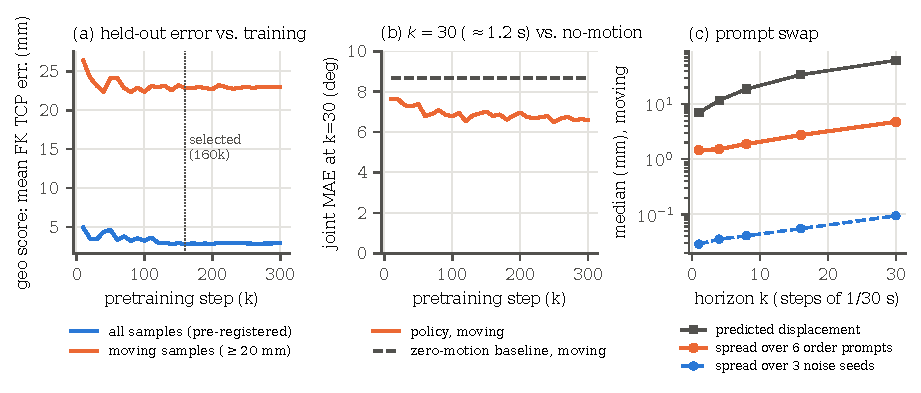
\includegraphics[width=\textwidth]{figures/fig4_eval.pdf}
\caption{Gen-1 오프라인 평가. (a) 학습 과정에 따른 전체 대 동작 held-out 샘플의 geo score. 사전 등록 규칙은 160k를 선택한다.
(b) 동작 샘플의 $k{=}30$ 관절 MAE, 정책 대 무동작 예측기. (c) 최종 체크포인트에 대한 prompt swap: 여섯 순서 지시문(같은 시드)
간 예측 퍼짐 대 세 노이즈 시드(올바른 지시문) 간 퍼짐.}
\label{fig:eval}
\end{figure*}

\textbf{학습 전 손실되는 데이터.} 후보 세그먼트의 57\%가 제거된다. 제거 745건 중 677건(91\%)이 작업공간 게이트에 의한 것이며, 그중
531건(78\%)에서는 한 팔만 로봇 작업공간을 벗어난다. 게이트가 동작의 범위로 동작을 제거하므로 남은 집합은 작은 동작 쪽으로 편향되었을
가능성이 높으나, 이 편향은 정량화하지 않았다. 리타게팅 v2(표~\ref{tab:retarget})가 이 손실의 상당 부분을 회복한다.

\textbf{로봇 파인튜닝을 위한 에고 사전학습.} 위의 에고 체크포인트와 base 체크포인트를 각각 같은 레시피·데이터·평가로 R150에서
파인튜닝하였다. 초기값만 다르다. 맞춘 스텝 250k에서 에고 초기화 모델은 geo score가 10.0\% 낮고(에피소드 수준 paired bootstrap,
10k회 추출: 95\% CI $-14.7$에서 $-5.6\%$), 동작 샘플 geo score가 7.2\% 낮으며(CI $-13.4$에서 $-1.8\%$), $k{=}30$ 동작 관절 MAE가
6.8\% 낮다(CI $-12.7$에서 $+0.5\%$). 평가 에피소드 10개 중 8개가 에고 초기화 쪽에 유리하다. 평가 에피소드는 두 파인튜닝 세트 모두에
포함되어 있으므로, 이는 일반화가 아니라 각 모델이 로봇 학습 분포에 얼마나 잘 맞는지를 측정한다. R90에서의 비교는 맞춘 스텝 두
개(10k, 20k)만 남기고 일찍 중단되었다. 여기서는 부호가 엇갈리므로(에고 초기화의 전체 샘플 geo $-33\%$와 $-11\%$, 동작 샘플 geo
$+2\%$와 $+13\%$) 결론을 내리지 않는다.

\textbf{최종 TR 데이터셋에서의 사전학습.} 996개 세그먼트 TR 데이터셋으로도 같은 레시피(계획 300k 스텝)를 써서 X-VLA를
사전학습하였다. 실행은 211.7k 스텝에서 중단되었고, 100k와 200k 체크포인트를 보관하며, 이들로부터의 로봇 파인튜닝 결과는 없다.

\section{결과: 데카르트 전이(Gen-2)}\label{sec:res2}
이 절의 모든 실행은 Gen-2 레시피를 쓰며, 로봇 데이터는 R312c이다.

\textbf{로봇 프레임에서의 에고 전용 모델.} 에고 데이터만으로 40k 스텝 학습한 뒤, 모델을 teacher forcing 방식으로 로봇 프레임 120개에
질의하고, 로봇 데이터로 40k 스텝 학습한 모델과 비교하였다(이 프레임들은 후자 모델의 학습 세트에 포함되므로 그 값은 상한 기준이다).
0.4\,s에서 예측 이동과 기록 이동 사이 코사인 중앙값은 로봇 모델이 $+0.81$/$+0.77$(왼쪽/오른쪽), 에고 모델이 $-0.05$/$-0.03$이다.
좌우 교환과 축 부호 반전의 어떤 조합도 에고 모델을 $+0.16$ 위로 올리지 못하며, 손목 카메라 광류는 두 도메인에서 TCP 동작과 같은
부호 관계를 가지므로, 이는 규약 오류가 아니다.

\begin{table}[t]
\centering\footnotesize\setlength{\tabcolsep}{3.2pt}
\caption{에고 전용 체크포인트(40k)에서 이미지와 상태가 서로 다른 도메인에서 올 때의 $k{=}4/8/16$ 방향 코사인 중앙값(왼쪽 $|$ 오른쪽).
에고 검증 프레임 100개와 로봇 프레임 100개, 셀당 동작 프레임 21--55개.}
\label{tab:ablation}
\begin{tabular}{@{}lcc@{}}
\toprule
이미지 + 상태 & 왼쪽 $k$=4/8/16 & 오른쪽 $k$=4/8/16 \\
\midrule
에고 + 에고 & 0.87 / 0.91 / 0.92 & 0.89 / 0.94 / 0.84 \\
에고 + 0 & 0.77 / 0.80 / 0.89 & 0.85 / 0.80 / 0.66 \\
에고 + 로봇 & 0.76 / 0.81 / 0.90 & 0.72 / 0.69 / 0.72 \\
로봇 + 로봇 & 0.36 / 0.30 / $-$0.01 & 0.19 / 0.02 / $-$0.15 \\
로봇 + 0 & 0.17 / 0.25 / $-$0.25 & 0.24 / 0.06 / $-$0.02 \\
로봇 + 에고 & 0.16 / 0.24 / $-$0.16 & 0.49 / 0.33 / $-$0.03 \\
\bottomrule
\end{tabular}
\end{table}

\textbf{격차는 이미지에 있다.} 표~\ref{tab:ablation}는 두 입력을 맞바꾼다. 에고 이미지를 주면 모델은 로봇 상태를 포함해 어떤 상태가
주어지든 0.69--0.90의 코사인을 유지하고, 로봇 이미지를 주면 상태와 관계없이 $-0.25$에서 $+0.49$ 사이로 떨어진다. 실패는 시각적이며,
이는 손목 시점의 30배 선명도 차이(\ref{sec:conv}절)와 부합한다.

\textbf{초기값으로서의 에고 사전학습(에피소드 312개).} R312c에서 base 모델(A)과 50k 스텝 에고 모델(B)로부터 동일한 데이터, 스케줄
(150k 스텝 cosine), 시드, 레시피로 파인튜닝하였다. 두 실행 모두 60k 근처에서 직접 중단하였다. 스텝 200에서 학습 손실은 A가 0.945,
B가 0.244이다. 비율 B/A는 처음 5k 스텝에서 0.49, 5k--20k에서 0.875, 20k--40k에서 0.95이며, 55k--60k에서는 두 값이 동률이다(0.0733 대
0.0745, 기록된 24개 지점 중 13개에서 B가 낮음)(그림~\ref{fig:egoinit}). 따라서 에고 사전학습은 로봇 데이터의 초기 피팅을 빠르게
하지만, 60k까지 학습 손실에서 측정 가능한 이점을 주지 않는다. 이는 조건당 시드 하나의 학습 손실이며, A와 B의 held-out 또는 폐루프
비교는 없다. 이후 300k 실행 두 개가 끝났으나 서로 다른 로봇 데이터셋(에고 초기화 실행은 R312c, scratch 실행은 R384)을 썼으므로 전이
비교가 아니다.

\begin{figure*}[t]
\centering
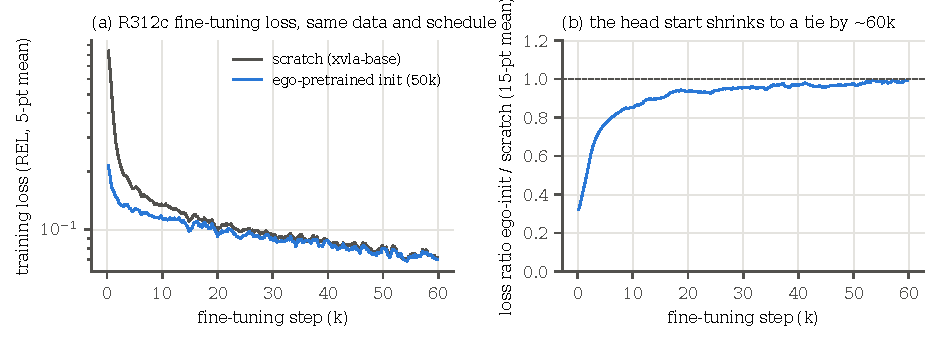
\includegraphics[width=\textwidth]{figures/fig5_ego_init_loss.pdf}
\caption{같은 데이터·스케줄·시드에서 base 모델과 50k 에고 체크포인트로부터의 R312c 파인튜닝 비교. (a) 학습 손실. (b) 둘의 비율.
1 미만이면 에고 초기화에 유리하다. 학습 손실만 해당.}
\label{fig:egoinit}
\end{figure*}

\textbf{시각적 격차를 줄이려는 시도.} \ref{sec:conv}절의 로봇 유사 렌더링을 모든 프레임에 적용하면(ROBOT100) 손목 선명도 중앙값은
1{,}854/1{,}487에서 181/132로 떨어지지만, 여전히 로봇의 59/64보다 두세 배 높다. 프레임의 70\%를 다시 렌더링한 실행은 5k 스텝에서
중단하였고, 배치마다 에고(ROBOT100) 샘플 네 개와 로봇 샘플 네 개를 쓰는 공동 학습 실행은 평가 없이 88.6k 스텝에서 중단하였다. 300k
ROBOT100 사전학습 실행(에피소드 297개, 행 48{,}411개, 49.6 epoch)은 10월 5일 학습 손실 0.007로 끝났으며, 그 체크포인트들이 다음
실험의 에고 초기값이다. 다시 렌더링한 모델에 대해서는 오프라인 전이 지표를 계산하지 않았다.

\textbf{저데이터 ablation: 로봇 에피소드 30개.} 312 에피소드 비교는 로봇 데이터가 초기값의 영향을 씻어 낼 여지를 충분히 준다. 인간
데이터 활용에 중요한 질문은 로봇 데이터가 부족할 때 도움이 되는지이다. R30으로, R312c 정규화 통계, seed 1000, 600k 스텝 cosine
스케줄을 써서 세 초기값에서 파인튜닝하였다. base 모델(scratch)과 ROBOT100 실행의 100k 및 300k 스텝이다. 100k 체크포인트는 같은 300k
스텝 스케줄의 중간에서 가져온 것이므로 학습률이 감쇠하지 않은 상태이며, 별도의 100k 스텝 실행이 아니다. 각 조건은 서로 다른 기계에서
실행되었으므로(scratch와 100k-init은 RTX~4090, PyTorch~2.6; 300k-init은 RTX~5090, PyTorch~2.7.1) 비트 단위로 동일한 쌍둥이 실행이
아니다.

\begin{table}[t]
\centering\footnotesize\setlength{\tabcolsep}{4pt}
\caption{R30 파인튜닝, 맞춘 스텝에서의 학습 손실(200스텝 이동 평균)과 scratch 대비 윈도 평균의 비율(1 미만이면 에고 초기화에 유리).
조건당 시드 하나, held-out 또는 로봇 평가 없음.}
\label{tab:r30}
\begin{tabular}{@{}lccc@{}}
\toprule
스텝 & Scratch & Ego-PT 100k 초기화 & Ego-PT 300k 초기화 \\
\midrule
200 & 0.801 & 0.239 & 0.446 \\
1k & 0.312 & 0.103 & 0.117 \\
10k & 0.065 & 0.056 & 0.040 \\
50k & 0.019 & 0.017 & 0.014 \\
100k & 0.009 & 0.009 & 0.007 \\
\midrule
윈도 & & 비율 & 비율 \\
\midrule
1k--5k & & 0.544 & 0.493 \\
10k--20k & & 0.823 & 0.697 \\
50k--100k & & 0.970 & 0.856 \\
100k--150k & & 1.021 & 0.914 \\
\bottomrule
\end{tabular}
\end{table}

표~\ref{tab:r30}와 그림~\ref{fig:r30}은 312 에피소드 비교와 같은 양상을 더 길게 늘여 보여 준다. 두 에고 초기화 모두 scratch 손실의
절반 미만에서 출발한다(1k--5k 윈도 비율 0.54와 0.49). 100k 스텝 초기화는 약 100k 스텝까지 이점을 잃고(50k--100k 비율 0.97,
100k--150k 비율 1.02), 300k 스텝 초기화는 더 작은 이점을 더 오래 유지하며(0.86과 0.91) 약 200k에서 동등해진다. 약 150k 이후로는 모든
손실이 출력 정밀도에서 0.001--0.004이므로 비율은 의미가 없다. 100k 스텝 초기화는 사전학습을 덜 했음에도 300k 스텝 초기화보다 낮게
출발하는데(스텝 200에서 0.239 대 0.446), 그 이유는 설명하지 못했다. 세 실행 모두 GPU를 비우기 위해 471k, 305k, 310k에서, 즉 214,
139, 141 epoch 후에 직접 중단하였다. 에피소드가 30개뿐이어서 모든 조건이 스케줄이 끝나기 훨씬 전에 학습 데이터에 거의 정확히 맞는다.
여기서 학습 손실은 각 초기값이 로봇 데이터를 얼마나 빨리 암기하는지를 측정할 뿐, 얼마나 잘 행동하는지를 측정하지 않는다. 의미 있는
비교는 초·중반 체크포인트(대략 10k--150k)에서의 폐루프 비교이며, R30 체크포인트는 아직 로봇에서 실행되지 않았다.

\begin{figure*}[t]
\centering
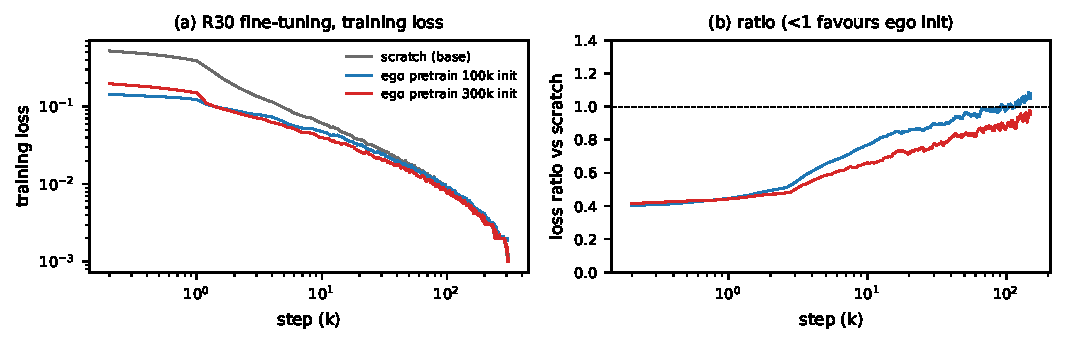
\includegraphics[width=0.8\textwidth]{figures/fig8_r30_ablation.pdf}
\caption{base 모델과 100k·300k 스텝 에고 사전학습으로부터의 R30 파인튜닝(로봇 에피소드 30개). (a) 학습 손실(log--log, 평활화).
(b) scratch 대비 비율, 150k까지 표시. 그 이후는 소수점 3자리 손실 때문에 비율이 노이즈가 된다. 학습 손실만 해당, 조건당 시드 하나.}
\label{fig:r30}
\end{figure*}

\section{결과: 단일 팔 접근}\label{sec:res3}
쌓기에서는 두 도메인이 하나의 액션 계약을 공유하면 남는 격차가 시각적·기하학적인 것임을 보였다. 큐브를 향한 단일 팔 접근은 훨씬 적은
교란 요인으로 이 격차를 따로 떼어 낸다. 팔 하나, 물체 하나, 파지 없음, 작업 순서 없음이며, 성공 여부를 눈으로 판단할 수 있다.

\textbf{HRA\_red (v1).} 200개 테이크 중 19개가 큐브 스케일 게이트에서 탈락하고(PnP 프레임 부족 14개, 퍼짐 과다 5개), 15개가 스케일을
적용한 궤적의 물리적 타당성 검사에서 탈락한다(스케일 0.1--1.0, SLAM 이동 거리가 PnP로 관측한 접근 거리의 0.8배 이상, 이동 거리
0.8\,m 이하). 남은 166개는 학습 에피소드 151개(20{,}319행)와 검증 에피소드 15개(2{,}011행)로 나눈다. 스케일 중앙값은 0.354(p5 0.188,
p95 0.500), 큐브 중심 잔차 중앙값은 0.17\,cm이다. 추정한 카메라 렌더링으로 한 300k 스텝 학습은 10월 5일 학습 손실 0.002(118 에폭)로
종료되었다. held-out 손실은 처음 평가한 체크포인트부터 상승한다(표~\ref{tab:val}, 그림~\ref{fig:val}a). 15k에서 0.150(학습 부분집합
0.066), 30k에서 0.198, 60k에서 0.213, 90k에서 0.265, 105k에서 0.299이며, 그동안 학습 부분집합 손실은 0.018까지 떨어진다. 에피소드
151개로는 모델이 거의 즉시 과적합한다.

\begin{table}[t]
\centering\footnotesize\setlength{\tabcolsep}{3pt}
\caption{체크포인트별 단일 팔 held-out 손실(지도되는 9차원에 대한 마스킹된 MSE). 괄호 안은 학습 부분집합 손실.}
\label{tab:val}
\resizebox{\columnwidth}{!}{\begin{tabular}{@{}lccccc@{}}
\toprule
데이터셋(검증 에피소드) & 5k & 15k & 30k & 45k/50k & 105k \\
\midrule
HRA\_red v1 (15) & -- & 0.150 (0.066) & 0.198 (0.053) & -- & 0.299 (0.018) \\
A100 A: 시작점 (11) & 0.124 (0.110) & 0.125 (0.058) & 0.141 (0.031) & 0.224 (0.020) & -- \\
A100 B: 원점 (11) & 0.132 (0.097) & 0.147 (0.057) & 0.174 (0.031) & 0.190 (0.022) & -- \\
\bottomrule
\end{tabular}}
\end{table}

\textbf{첫 로봇 실행과 그로써 드러난 것.} 10월 4일 v1 15k--75k 체크포인트로 8{,}397 제어 사이클(실행 시작 658회)을 돌렸고, 10월 6일에는
청크 실행 설정을 조정하면서 100k, 200k, 300k로 계획 세션 61개를 실행했다. 작업자의 평가는 ``정확도가 많이 떨어졌다'', ``지그재그가
너무 심하다''였다. 큐브 가까이에서 시작하면 팔은 큐브를 향해 움직였고, 왼쪽으로 멀리 놓인 큐브에 대해서는 두 번의 실행에서 각각 약
39\,cm, 26\,cm 테이블 위를 끌며 이동했다. 이 실행들을 해석하려면 인간 데이터가 로봇에 대해 어디에 위치하는지 알아야 했지만, v1은
이를 전혀 다루지 않았다. v1의 레이블은 UMI 도구 좌표계의 상대 운동이고, 시작 상태는 인간 자신의 시작 자세이기 때문이다. 테이크를
사후에 로봇 베이스에 연결하는 방법(헤드 카메라의 큐브, 큐브 PnP를 통한 손목 궤적, IMU 중력에서 얻은 기울기)은 166개 테이크 중 64개만
연결했으며, 시작 높이가 4\,cm 범위로 퍼지고 상방 축 오차가 p50 10\textdegree, p90 28\textdegree{}였다. 또한 이 과정에서
\ref{sec:pose}절의 18\textdegree{} 카메라--IMU 오류가 드러났다. 테이크 시작 시점의 인간 손목 카메라와 도달 가능한 시작 자세에서의 로봇
손목 카메라는 일치시킬 수 없다. 인간의 시점을 맞추려면 어깨 관절이 한계를 넘어야 하기 때문이다. 가장 가까운 실현 가능한 시작 자세(자세
A)에서 카메라는 수평면 내에서는 1--14\mm{} 이내이지만, 78\mm{} 더 높고 8\textdegree{} 더 가파르다. 자세 A와 조 끝단 모델을 사용하여,
v1 200k를 세 가지 도구 좌표계 규약으로 다시 읽은 결과는 다음과 같다. 도구 축을 회전하지 않으면 끝단은 큐브에서 약 2\,cm, 테이블 위
3\,cm에서 멈췄다. 카메라 피치 33.1\textdegree{}만큼 회전하면 약 11\,cm 지나쳤다. 회전과 함께 카메라--TCP 병진만큼 오프셋하면 큐브에서
약 4\,cm, 테이블 위 10\,cm에서 멈췄다. 이는 FK로 재구성한 단일 실행이며, 성공을 측정한 것이 아니다. robotcam v2로 한 학습은 약 64k
스텝(학습 손실 0.026)에서 중단되었다.

\textbf{HRA\_A100: 공유 원점.} 각 테이크는 자동 사이클로 진행된다(그림~\ref{fig:protocol}). 5\,s 휴식 후, 작업자가 HandUMI 조 끝단을
테이프 십자 위에 놓고 2\,s 동안 정지시킨다. 녹화는 추가 2\,s 홀드(원점)로 시작한다. 3\,s ``준비'' 단계에서 손을 로봇과 비슷한 시작
자세로 옮기고, ``go'' 신호에 10\,s 접근을 녹화하며, 학습 데이터는 ``go''부터 시작한다. 큐브 배치는 중앙 40, 좌/우 20, 앞/뒤 20,
가장자리 20으로 계획했다. 10월 6일 네 세션에서 107개 테이크를 확보했다(7, 8, 9, 83개. 첫 세션은 원점 홀드 도입 이전이다). 스케일은
큐브 PnP 또는 원점 평면에서, 좌표계와 yaw는 G에서 얻는다(\ref{sec:pose}--\ref{sec:conv}절).

\begin{figure}[t]
\centering
\begin{tikzpicture}[font=\scriptsize, x=0.375cm]
\foreach \a/\b/\t/\c in {0/5/휴식/black!8, 5/7/정지/orange!20, 7/9/홀드/orange!45, 9/12/준비/blue!12, 12/22/접근(학습 데이터)/blue!30}
  {\fill[\c] (\a,0) rectangle (\b,0.55); \draw[black!50] (\a,0) rectangle (\b,0.55); \node at ({(\a+\b)/2},0.27) {\t};}
\foreach \x/\l in {0/0, 5/5, 7/7, 9/9, 12/12, 22/22\,s} \node[below] at (\x,0) {\l};
\end{tikzpicture}
\caption{HRA\_A100 테이크 사이클: 휴식, 테이프 십자 위에 조 끝단 정지, 2\,s 원점 홀드로 녹화 시작, 준비, 10\,s 접근.
원점 홀드는 HandUMI 조 끝단을 캘리브레이션 시 로봇 조 끝단이 터치했던 것과 같은 테이프 십자 위에 놓는다.}
\label{fig:protocol}
\end{figure}

\textbf{시작점 기준 대 원점 기준 상태.} 93개 테이크(학습 82, 검증 11. 제외된 14개는 이전 세션, 홀드 중 손이 20\mm{} 넘게 움직인 테이크
7개, 물리 검사 실패 한 개)로, 다른 조건은 모두 같은 두 모델을 학습했다. A는 ``go'' 시점의 손 자세를 상태의 기준으로, B는 고정된 원점
좌표계 F(십자 위치, 테이프 방위, 홀드 피치 중앙값)를 기준으로 삼는다. 둘 다 로봇 TCP 레이블과 robotcam v2 렌더링을 사용한다. 두
모델의 held-out 손실은 비슷하며 둘 다 첫 체크포인트에서 가장 낮다(표~\ref{tab:val}, 그림~\ref{fig:val}b). 5k에서 A 0.124, B 0.132이고,
0.224(A, 50k), 0.190(B, 45k)까지 상승한다. 학습 테이크 82개로는 두 모델 모두 5k 스텝부터 과적합한다. 이 지표로는 어느 기준도 더
낫지 않다.

\begin{figure*}[t]
\centering
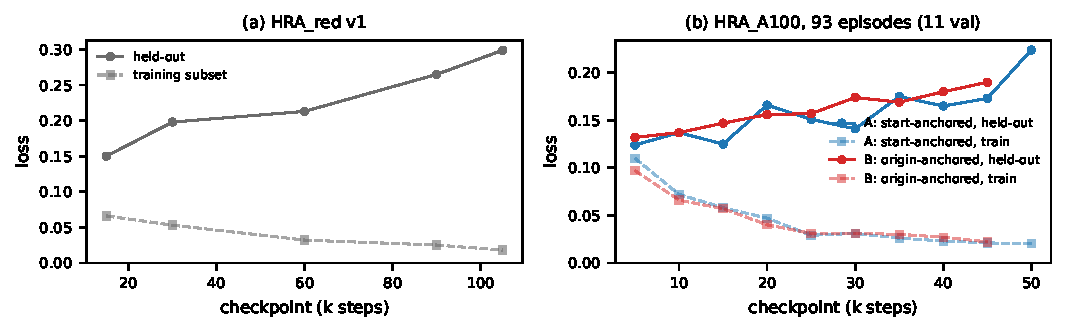
\includegraphics[width=0.8\textwidth]{figures/fig9_hra_val.pdf}
\caption{체크포인트별 held-out 손실(실선)과 학습 부분집합 손실(점선). (a) HRA\_red v1, 검증 테이크 15개. (b) HRA\_A100,
시작점 기준(A) 및 원점 기준(B) 상태, 검증 테이크 11개. 모든 실행이 가장 이른 체크포인트부터 과적합한다.}
\label{fig:val}
\end{figure*}

\textbf{시작 자세.} G에서 인간 ``go'' 자세의 중앙값과 메도이드로부터 뒤, 오른쪽, 아래로 옮겨 도출한 로봇 시작 자세 후보 열 개를
비교했다. 작업자는 가장 낮은 자세(자세 08, TCP $(273, -168, 116)$\mm, 관절 여유 9.1\textdegree)를 선호했다. 10월 7일에는 더 낮은 인간
시작 자세로 27개 테이크를 추가 녹화했으나(원점에서 ``go''까지 약 247\mm{} 대신 약 89\mm), 자세 08 기준으로 5개만 통과하여 제외했다.
따라서 현재 학습(CT7-old, 10월 6일 테이크 85개, 시작 자세 08, 100k 스텝 스케줄)은 10월 6일 데이터만 사용한다. CT5와 CT6 학습은 설정이
바뀌는 동안 각각 7k, 3k 스텝에서 중단되었으며, CT6와 CT7에는 검증 분할이 없다.

\section{배포와 로봇 관찰}\label{sec:deploy}
\textbf{추론과 제어.} 정책은 Mac(Apple 실리콘 GPU, bf16)에서 디노이징 스텝 5회(양팔) 또는 10회(단일 팔)로 실행된다. 로봇 카메라는
640$\times$480으로 캡처하고 224$\times$224로 크기를 맞추어 학습과 같이 정규화한다. 단일 팔 모드에서는 왼 손목 이미지가 검은색이다.
상태는 학습 계약을 따른다(측정 관절의 FK로 구한 TCP 자세를, 실행 시작 시 잡은 앵커 또는 고정 앵커 파일 기준 상대 자세로 표현). 절대
목표 $T_k=T_\text{now}A_k$는 URDF에 대해 Pink~\cite{caron2024pink} IK로 푼다. \emph{PLAN mode}에서는 순전파 하나를 항상 진행 중으로
유지하면서 IK로 푼 행(50.05\,ms 간격)을 로봇 서비스로 스트리밍하고, 로봇 서비스는 이를 MIT impedance mode에서 100\,Hz 보간점(knot)으로
재생한다. 계획된 보간점이 90\textdegree{} 넘게 튀면 팔을 정지시킨다. 선택적인 real-time chunking~\cite{black2025rtc}은 각 새 청크를
이전 청크의 아직 실행되지 않은 목표 쪽으로 끌어당긴다.

\textbf{중요했던 설정.} (i) \emph{청크 실행}: 연속된 16스텝 청크를 블렌딩한다. 지수 블렌드 0.25, 크로스페이드 없음, 스무딩 없음,
청크당 최소 실행 행 한 개일 때 동작은 수용할 만했다. 반면 10월 7일 인터페이스 재시작 시 조용히 되돌아간 코드 기본값(0.35, 4행,
3\textdegree, 6행)에서는 작업자가 ``추론 품질이 많이 낮아졌다''고 보고했고, 이는 값을 복원할 때까지 지속되었다. 로봇에서의 거동은
체크포인트에 포함되지 않는 설정에 좌우되며, 현재는 로더가 이 설정을 복원한다. (ii) \emph{도구 좌표계 규약}: 로봇 TCP 레이블로 학습한
모델(robotcam v2, A100)은 카메라 피치 0, 카메라--TCP 오프셋 0으로 실행해야 한다. 33.1\textdegree{} 피치와 오프셋은 v1에만 적용되며,
기준 고정(anchored) 모델은 같은 앵커 파일(B는 F, CT5--CT7은 G)로 서빙해야 한다. (iii) \emph{큐브 크기 정지}: 팔이 멈추지 않고 큐브를
미는 것이 관찰된 뒤, 인터페이스는 0.1\,s마다 빨간 큐브의 겉보기 크기(원본 640$\times$480 손목 프레임에서 픽셀 단위
$\sqrt{\text{area}}$)를 측정하고, 두 번의 측정값이 임계값(170--250\,px 사용)을 넘으면 정지한다. 팔로우 모드(follow mode)에서는 큐브가
임계값의 85\% 미만으로 작아지면 재개한다. 이는 근접 대리 지표이지 검증된 접촉이 아니다. 또한 같은 위치에서 큐브가 학습 때보다 작게
보였기 때문에 손목 영상을 1.5$\times$ 확대했다. (iv) \emph{안전 장치}: v1 동안 인터페이스는 순 이동 450\mm, 추론 간 이동 80\mm, 정지
구간, 또는 250\mm{}나 60\textdegree{}를 넘는 출력이 발생하면 실행을 중단했다. 6\,s 시간 제한은 1--4 사이클 만에 실행을 끝내 버려
제거했다. A100 모델에서는 모든 수치 안전 장치를 끄고, 왼팔과 조는 잠근 상태로 둔다.

\textbf{로봇에서의 쌓기.} Gen-2 체크포인트를 배포 인터페이스를 통해 reBot에서 실행하였다. 10월 2일에서 4일 사이에 체크포인트 71개,
제어 사이클 49{,}431회, 실행 시작 1{,}681회이다. 사이클 로그는 과제 결과가 아니라 모델 자신의 웨이포인트에 대한 IK 추적을 기록하므로
성공률을 산출할 수 없다. 조작자의 관찰 두 가지는 로그로 남지 않았다. 파인튜닝 10k 스텝의 에고 초기화 모델은 큐브를 잡았으나 틀린 색을
집었다. R312c로 300k 파인튜닝한 에고 초기화 모델(B300, 75k에서 205k 사이의 체크포인트)은 폐루프로 큐브 세 개를 끝까지 쌓았다. 시도
횟수는 기록되지 않았고 영상도 찍지 않았으므로, 폐루프 큐브 삼단 쌓기가 시연되었다는 사실만 말할 수 있으며 성공률은 없다. 이는 에고
사전학습의 가치에 대해서도 아무것도 말해 주지 않는다. R312c로 학습한 scratch 모델은 같은 프로토콜로 평가되지 않았다. 큐브를 쌓은
B300 체크포인트 중 저장소 정리 후 남은 것은 150k와 200k뿐이므로, 시연은 이들로부터만 재현할 수 있다. 시도 로거(체크포인트, 로봇
데이터, 지시문, 배치, 쌓기 단계 0--3, 틀린 색, 실패 원인)가 10월 4일 추가되었으나 사용되지 않았다.

\textbf{로봇에서의 접근.} 계획 실행 로그에는 10월 6일과 7일에 걸쳐 192개 세션이 기록되어 있다. 10월 6일의 65개 세션(v1 체크포인트,
앞서 기술한 청크 설정 조정)은 하나를 제외하고 모두 작업자가 중단했으며, 그 하나는 계획된 행이 90.9\textdegree{} 튀어 인터페이스가
종료했다. 10월 7일에는 127개 세션이 실행되었다. B 45k(3), A 50k(6), CT5 5k(4)에 이어 1.5$\times$ 확대를 적용한 B 50k(114개 세션, 다수가
팔로우 모드 재개)를 실행했다. 127개 중 69개는 큐브 크기 정지로, 58개는 작업자 중단으로 끝났다. 로그에는 결과 필드가 없으므로 몇 번의
접근이 큐브에 도달했는지 말할 수 없다. 큐브는 어안 영상으로 렌더링한 학습 이미지에서는 주황색으로, 로봇 카메라에서는 빨간색으로
보이는데, 이 색 격차는 보정하지 않았다.

\section{수정 사항과 알려진 불일치}\label{sec:corr}
우리 자신의 중간 판독 중 여러 개가 틀렸으며, 각각 독립적인 검사로 발견되었다. 로봇 시작 기울기는 3\textdegree{}가 아니라
25\textdegree{}였다. 로봇의 손목 뷰는 인간보다 2.5$\times$가 아니라 약 1.32$\times$ 확대되어 있고 11\textdegree{} 낮다. ``레이블이
끝단을 테이블 속 5\,cm까지 밀어 넣는다''는 판독은 TCP--끝단 오프셋 때문이었다. 테이블 높이는 접촉 모델을 고치면서 $-54.3$에서
$-5.9$, 다시 $-27.1$\mm{}로 바뀌었다. IMU 기울기 통계는 최대 18\textdegree{} 틀려 있었다. 평균 원점 yaw는 잘못된 기각을 일으켰다.
이전 내보내기의 카메라 방향 규약 오류는 프레임 회귀 테스트로 발견되기 전까지 회전을 손상시켰다. 그리고 우리 embodiment id 두 개는
학습되지 않은 soft prompt를 가리키고 있었다.

이 보고서를 작성하면서 우리 코드의 불일치도 드러났으며, 숨기지 않고 나열한다. (1) 팔 간 간격 검사는 Gen-1 게이트가 아니라 리타게팅
v2에서만 쓰인다. (2) Gen-1 목표 코드에서 이진화된 그리퍼 레이블 1은 주석에는 닫힘이라고 되어 있지만 실제로는 \emph{열림}을 뜻한다.
(3) 그리퍼 캘리브레이션이 세 가지 사용된다(67.5\mm{} 개구의 Gen-1 tick, Gen-2의 gcal1 캘리퍼 보간점, 수집기의 열림/닫힘 파일). 각
데이터셋은 자신이 쓰는 것을 명시한다. (4) 내보내기 도구가 쓰는 카메라--IMU 시간 오프셋은 raw 캘리브레이션 출력과 부호와 크기가
다르며, 이를 변환한 단계는 기록되어 있지 않다. (5) 내보내기 도구와 한 뷰어 도구가 서로 다른 두 버전의 오른쪽 어안 캘리브레이션을
사용한다. (6) IK 스텝 임계값은 15\,Hz 행 기준으로 문서화되어 있으나 30\,fps 행에 적용된다. (7) PLAN mode에서 양팔 경로는 그리퍼 폭을
웨이포인트 솔버에 전달하지 않으므로 조가 닫힌 채로 남을 가능성이 높다. 조를 고정하는 단일 팔 실행은 영향을 받지 않는다. (8) 여러
진단은 저장소 밖의 스크립트로 실행되었으며, 그 출력은 다시 실행한 것이 아니라 캡처한 로그로 보관되어 있다. (9) G 프레임, 손끝 박스,
18\textdegree{} 카메라--IMU 보정의 피팅 스크립트는 저장소에 없고 그 출력만 있다.

\section{교훈}\label{sec:lessons}
다음 각각은 손실 곡선이 아니라 명시적인 검사로 발견되었다. (i) \emph{모든 자세 또는 스케일 원천에는 드러나지 않게 실패하는 영역이
있다}. 장면 변경을 넘는 ORB-SLAM3, 드문 한 프레임 점프에서의 MASt3R-SLAM, 느린 동작에서의 IMU, 비스듬한 단일 면 뷰에서의 큐브 PnP,
일부 테이크에서의 원점 평면(p90 오차 37\%)이 그렇다. 실패는 독립적인 두 번째 기준이 있어야만 드러난다. (ii) \emph{사전학습 모델의
조건화 인터페이스는 가정하지 말고 점검해야 한다}. 본 연구의 embodiment id 두 개는 한 번도 학습된 적 없는 soft prompt를 가리키고
있었다. (iii) \emph{인간 데이터와 로봇 데이터가 텐서 계약을 공유하면, 도메인 간 입력을 맞바꾸어 남은 격차의 위치를 찾을 수 있다}.
여기서는 기구학이나 정규화가 아니라 손목 이미지였다. (iv) \emph{공유된 물리적 원점은 사후 정합보다 저렴하다}. 테이크를 사후에
연결한 결과는 센티미터 단위 오차로 166개 중 64개에 그쳤지만, 로봇과 인간이 모두 터치한 테이프 십자는 서브밀리미터 수준의 직선
피팅으로 공통 좌표계를 제공한다. (v) \emph{IK 스택의 TCP는 규약일 뿐 손끝이 아니다}. 접촉을 추론하려면 손끝 형상이 필요하다.
(vi) \emph{초기값 간 학습 손실 비교는 로봇 데이터가 거의 0까지 피팅될 때마다 동률로 끝난다}. 312개와 30개 에피소드 모두 그랬으며,
작은 단일 과제 데이터셋은 즉시 과적합한다. 이점은 초기 체크포인트에서의 held-out 또는 폐루프 평가로만 보일 수 있다. (vii) \emph{실행
설정은 정책의 일부이다}. 인터페이스에 있는 블렌드·스무딩 파라미터가 체크포인트 교체보다 로봇 거동을 더 크게 바꾸었으며, 결과
로깅은 로봇 실행 후가 아니라 그 전에 갖춰져 있어야 한다.

\section{한계 및 향후 연구}\label{sec:lim}
\textbf{조기 중단, 결론 없음:} R90 파인튜닝 비교(맞춘 스텝 두 개), 70\% 재렌더링 사전학습(5k 스텝), 에고/로봇 공동 학습 실행(88.6k
스텝, 평가하지 않음), robotcam v2 실행(64k), CT5/CT6 실행. \textbf{미수행:} 996 세그먼트 체크포인트로부터의 로봇 파인튜닝, R30
조건들의 로봇 또는 held-out 평가, 에고 초기화 모델과 scratch 모델의 held-out 또는 폐루프 비교, 로봇에서의 결과 로깅.

\textbf{본 연구가 뒷받침하지 않는 것:} (i) 쌓기나 접근의 폐루프 성공률, 또는 에고 초기화 모델과 scratch 모델 간의 폐루프 차이,
(ii) 새 큐브 배치로의 일반화(배치를 기록하지 않았고 Gen-1은 설계상 절대 기하를 버림), (iii) 보지 못한 쌓기 순서로의 일반화(여섯 순서
모두 학습에 등장), (iv) 조작자 한 명, 장면 하나, 며칠을 넘어서는 전이, (v) 로봇 학습 분포를 더 빨리 피팅하는 것 이상의 인간 데이터
이점, (vi) 에고 전용 정책 또는 재렌더링한 손목 이미지가 로봇 카메라로 전이된다는 것, (vii) 접근 데이터에서의 색 그라운딩.

\textbf{계획된 실험:} 실행 설정을 고정한 채 모든 로봇 시도를 기록하고(모델, 체크포인트, 로봇 데이터 크기, 시작 자세, 배치, 지시문,
쌓기 단계 0--3 또는 도달 여부, 실패 및 정지 사유) 모델당 20--30회 시도한다. scratch 모델과 에고 초기화 모델을 맞춘 파인튜닝 스텝과
R30에서 비교하여 쌓기가 처음 성공하는 스텝 및 데이터 예산을 찾는다. A, B, CT7의 이른 접근 체크포인트(5k--15k)를 같은 시작 자세와
큐브 위치에서 시험한다. 헤드 카메라로 배치를 기록하고 배치 영역을 held-out으로 둔다. 두 순서를 완전히 held-out으로 두고 지시문
추종을 검증한다. 렌더링된 손목 영상의 색을 보정한다. 정지 구간을 고려한 손실로 학습한다. 그리고 접근 사전(prior)을 쌓기 정책의 첫
구간으로 사용한다.

더 넓게 보면, 본 연구는 에고센트릭 인간 시연을 로봇 정책을 위한 확장 가능한 지도 신호로 쓰기 위한 첫걸음이다. 즉 embodiment 세부는
버리고 과제 기하와 의도는 유지하는 인간--로봇 표현을 학습하고, 실행 전에 예측 world model로 이를 평가하는 것이다. 현재 결과는 병목이
정책 못지않게 자세 복원, 필터링, 캘리브레이션, 평가 설계에 있음을 보여 준다.

\section{결론}
업스트림 오픈소스 손 착용 그리퍼에 손목 IMU를 추가하여 제작하고, 양팔 쌓기 시연 349개와 단일 팔 접근 데이터셋 두 개를 수집하여 두
가지 방식으로 로봇 학습 데이터로 바꾸었다. 로봇 관절로 리타게팅한 쌓기 데이터는 0.9B VLA에 held-out 인간 동작의 방향을 가르치지만
(동작 샘플에서 $k{=}30$ 코사인 0.90) 순서 지시문의 사용은 가르치지 못하며, 정지 구간 드리프트는 집계 지표에 가려진다. 다중 시드 궤적
검색은 리타게팅 손실의 상당 부분을 없앤다. 로봇 자신의 데카르트 계약으로 변환하면, 드러나지 않는 SLAM 점프를 제거한 뒤 실현 가능성
필터 없이 에피소드 전체가 남으며, 남은 인간--로봇 격차는 시각적이고 손목 이미지에 있다. 초기값으로서 에고 사전학습은 로봇 에피소드
312개와 30개 모두에서 초기 로봇 파인튜닝을 빠르게 하며, 학습 손실상의 이점은 로봇 데이터가 피팅되면서 사라진다. 에고 초기화 모델이
로봇에서 큐브 세 개를 끝까지 쌓았으므로 과제 자체는 폐루프로 해결되었다. 에고 사전학습이 더 적은 로봇 에피소드나 스텝으로 그 지점에
도달하는지는 열린 질문이다. 느린 단일 팔 동작에서는 알려진 물체와 공유된 물리적 원점이 IMU 스케일을 대신하여 인간 데이터를
서브센티미터 수준의 일관성으로 로봇 좌표계에 들여온다. 이러한 테이크 80--150개로 학습한 모델은 빠르게 과적합하며, 가까운 시작점에서
큐브를 향해 움직인다. 측정된 성공률, 공간 및 과제 순서 일반화, 겹치지 않는 로봇 데이터에서의 이점에는 위에 나열한 통제 실험이
필요하다.

\appendices
\section{코드 맵과 보고서 이력}\label{app:code}
\textbf{코드 맵}(저장소 내 경로): 수집기와 프로토콜 \code{collection/} (\code{autoloop.py}, \code{recorder.py},
\code{integrity.py}); 하드웨어와 IMU 펌웨어 \code{hardware/}, \code{collection/firmware/}; 업스트림 라이선스, NOTICE, 우리의 패치
\code{upstream/}; 내보내기와 동기화 \code{pipeline/export/}, \code{pipeline/census/}; MASt3R-SLAM 래퍼와 스케일
\code{pipeline/mast3r_pose/}, \code{cart20/ego_cart20/cube_pnp.py}; Gen-1 \code{pipeline/pseudo_joint/}, \code{pipeline/retarget_v2/};
Gen-2 \code{cart20/}(계약, 자세 필터, 변환기, 검증기); 단일 팔 \code{hra/}; 학습 \code{training/}; 평가와 진단 \code{evaluation/},
\code{analysis/}; 배포 \code{deploy/}; 주장 검증 \code{analysis/verify_claims.py}.

\textbf{보고서 이력.} 버전 2(2026년 9월 30일)는 Gen-1 쌓기를 다루었고, 버전 3(10월 4일)은 Gen-2와 전이 진단을 추가하였으며, 버전
4(10월 7일)는 R30 ablation을 추가하고 작업을 제I부(쌓기), 제II부(접근), 방법 문서로 나누었다. 버전 4.1(10월 12일)은 하드웨어 설명을
추가하였다. 이번 버전 5는 어떤 결과도 바꾸지 않고 이들을 하나의 보고서로 합친 것이며, 이전 문서들은 저장소에 남아 있다.

\begin{thebibliography}{99}\footnotesize
\bibitem{chi2024umi} C.~Chi, Z.~Xu, C.~Pan, E.~Cousineau, B.~Burchfiel, S.~Feng, R.~Tedrake, and S.~Song, ``Universal manipulation interface: In-the-wild robot teaching without in-the-wild robots,'' in \emph{RSS}, 2024.
\bibitem{wang2024dexcap} C.~Wang, H.~Shi, W.~Wang, R.~Zhang, L.~Fei-Fei, and C.~K. Liu, ``DexCap: Scalable and portable mocap data collection system for dexterous manipulation,'' in \emph{RSS}, 2024.
\bibitem{ohkawa2026yubi} T.~Ohkawa, J.~Arima, Y.~Noguchi \emph{et al.}, ``YUBI: Yielding universal bidigital interface for bimanual dexterous manipulation at scale,'' arXiv:2606.10244, 2026.
\bibitem{handumi_hw} BrikHMP18 and HandUMI contributors, ``HandUMI: Hardware,'' GitHub repository, \url{https://github.com/murobotics-ai/handumi-hw} (first published as \texttt{robonet-ai/handumi-hw}), Apache-2.0, 2026. Commit \texttt{e58de33} used.
\bibitem{handumi_sw} BrikHMP18 and HandUMI contributors, ``HandUMI: Software,'' GitHub repository, \url{https://github.com/murobotics-ai/handumi-sw} (first published as \texttt{robonet-ai/handumi-sw}), Apache-2.0, 2026. Commit \texttt{33cc437} used.
\bibitem{kareer2024egomimic} S.~Kareer \emph{et al.}, ``EgoMimic: Scaling imitation learning via egocentric video,'' \emph{arXiv:2410.24221}, 2024.
\bibitem{wang2023mimicplay} C.~Wang \emph{et al.}, ``MimicPlay: Long-horizon imitation learning by watching human play,'' in \emph{CoRL}, 2023.
\bibitem{grauman2022ego4d} K.~Grauman \emph{et al.}, ``Ego4D: Around the world in 3,000 hours of egocentric video,'' in \emph{CVPR}, 2022.
\bibitem{zhao2023act} T.~Z. Zhao, V.~Kumar, S.~Levine, and C.~Finn, ``Learning fine-grained bimanual manipulation with low-cost hardware,'' in \emph{RSS}, 2023.
\bibitem{chi2023diffusion} C.~Chi, S.~Feng, Y.~Du, Z.~Xu, E.~Cousineau, B.~Burchfiel, and S.~Song, ``Diffusion policy: Visuomotor policy learning via action diffusion,'' in \emph{RSS}, 2023.
\bibitem{kim2024openvla} M.~J. Kim \emph{et al.}, ``OpenVLA: An open-source vision-language-action model,'' in \emph{CoRL}, 2024.
\bibitem{black2024pi0} K.~Black \emph{et al.}, ``$\pi_0$: A vision-language-action flow model for general robot control,'' \emph{arXiv:2410.24164}, 2024.
\bibitem{zheng2025xvla} J.~Zheng \emph{et al.}, ``X-VLA: Soft-prompted transformer as scalable cross-embodiment vision-language-action model,'' in \emph{ICLR}, 2026 (arXiv:2510.10274).
\bibitem{cadene2024lerobot} R.~Cadene \emph{et al.}, ``LeRobot: State-of-the-art machine learning for real-world robotics in PyTorch,'' \url{https://github.com/huggingface/lerobot}, 2024.
\bibitem{lipman2023flow} Y.~Lipman, R.~T.~Q. Chen, H.~Ben-Hamu, M.~Nickel, and M.~Le, ``Flow matching for generative modeling,'' in \emph{ICLR}, 2023.
\bibitem{murai2025mast3rslam} R.~Murai, E.~Dexheimer, and A.~J. Davison, ``MASt3R-SLAM: Real-time dense SLAM with 3D reconstruction priors,'' in \emph{CVPR}, 2025.
\bibitem{furgale2013kalibr} P.~Furgale, J.~Rehder, and R.~Siegwart, ``Unified temporal and spatial calibration for multi-sensor systems,'' in \emph{IROS}, 2013.
\bibitem{tsai1989handeye} R.~Y. Tsai and R.~K. Lenz, ``A new technique for fully autonomous and efficient 3D robotics hand/eye calibration,'' \emph{IEEE Trans. Robotics and Automation}, 1989.
\bibitem{xiao2024florence2} B.~Xiao \emph{et al.}, ``Florence-2: Advancing a unified representation for a variety of vision tasks,'' in \emph{CVPR}, 2024.
\bibitem{caron2024pink} S.~Caron \emph{et al.}, ``Pink: Python inverse kinematics based on Pinocchio,'' \url{https://github.com/stephane-caron/pink}, 2024.
\bibitem{black2025rtc} K.~Black, M.~Y. Galliker, and S.~Levine, ``Real-time execution of action chunking flow policies,'' \emph{arXiv:2506.07339}, 2025.
\end{thebibliography}
\end{document}
